\pdfoutput=1
\documentclass{article}
\usepackage{pack}
\usepackage[backend = bibtex, sorting = none]{biblatex}
\addbibresource{biblio.bib}

\usepackage{lineno}
%\linenumbers

\title{Computing character tables and Cartan matrices of finite monoids with fixed point counting.}

\author{Balthazar Charles\footnote{LISN, Université Paris-Saclay, 6 Rue Noetzlin, Gif-sur-Yvette, 91190, France}}
\date{}

\begin{document}
	
	%\begin{frontmatter}
		
		\maketitle
						
		\begin{abstract}
			%% Text of abstract
			In this paper we present an algorithm for efficiently counting fixed points in a finite monoid $M$ under a conjugacy-like action. We then prove a formula for the character table of $M$ in terms of fixed points and radical, which allows for the effective computation of the character table of $M$ over a field of null characteristic, as well as its Cartan matrix, using a formula from [Thiéry '12], again in terms of fixed points. We discuss the implementation details of the resulting algorithms and provide benchmarks of their performances.
		\end{abstract}
		
	%\end{frontmatter}
	
	\section*{Introduction}
	
	\section{Introduction}

The increasing complexity of source code poses a key challenge to the reliability of large-scale software systems. Software bugs in these systems can lead to safety issues~\cite{bug_safety} for users around the world as well as cause non-negligible financial losses~\cite{bug_loss}. As such, developers have to spend a large amount of time and effort on bug fixing. Consequently, \aprfull (\apr), designed to automatically generate patches to fix software bugs, has attracted wide attention from both academia and industry~\cite{long2016prophet, legoues2012genprog, long2015spr, lou2020can, tufano2018empstudy}. 


To achieve \apr, one popular approach is known as Generate-and-Validate (G\&V)~\cite{qi2015gv, ghanbari2019prapr, lou2020can, le2016hdrepair, legoues2012genprog, wen2018capgen, hua2018sketchfix, martinez2016astor, koyuncu2020fixminder, liu2019tbar, liu2019avatar}, which is typically based on the following pipeline: First, fault localization techniques~\cite{wong2016fl, abreu2007ochiai, zhang2013injecting, papadakis2015metallaxis, li2019deepfl, li2017transforming} are applied to determine the suspicious locations in programs where bugs are likely to exist. Then, the buggy locations are used by the \apr tools to generate a list of patches that replace buggy lines with correct lines. Afterward, each patch is validated against the original test suite to identify any \emph{plausible patches} (i.e., passing all tests in the test suite). Finally, to determine the \emph{correct patches}, developers examine the list of plausible patches to see if any of them can correctly fix the bug. 

Traditional \apr tools can mainly be categorized into heuristic-based~\cite{legoues2012genprog, le2016hdrepair, wen2018capgen}, constraint-based~\cite{mechtaev2016angelix, le2017s3, demacro2014nopol, long2015spr} and \template~\cite{ghanbari2019prapr, hua2018sketchfix, martinez2016astor, liu2019tbar, liu2019avatar}. Among these traditional tools, \template \apr tools~\cite{ghanbari2019prapr, liu2019tbar, benton2020effectiveness} have been able to achieve state-of-the-art results. \Template \apr tools typically leverage pre-defined templates (e.g., adding a nullness check) for bug fixing. However, since these fix templates are typically handcrafted, the number and types of bugs they are able to fix can be limited. 



To address the limitations of traditional \apr, researchers have proposed various \learning \apr tools~\cite{li2020dlfix, chen2018sequencer, jiang2021cure, lutellier2020coconut, zhu2021recoder, ye2022rewardrepair} based on the \nmtfull (\nmt) architecture~\cite{sutskever2014mt} where the input is the buggy code snippets and the goal is to translate the buggy code snippets into a fixed version. To accomplish this, \learning \apr tools require supervised training datasets with pairs of both buggy and fixed code snippets in order to learn how to perform this translation step. These training data are usually obtained by mining historical bug fixes using heuristics/keywords~\cite{dallmeier2007benchmark}, which can be imprecise for identifying bug-fixing commits; even the actual bug-fixing commits can include irrelevant code changes, leading to further pollution in the dataset~\cite{xia2022alpharepair}.
% 
Moreover, it can be hard for such \apr tools to generalize and fix bug types unseen during training. 



To better leverage recent advances in \plmfull{s} (\plm{s}), researchers~\cite{xia2022alpharepair, xia2023repairstudy, kolak2022patch, prenner2021codexws} have directly applied \plm{s} to generate patches without bug-fixing datasets. These \llm-based \apr tools work by either directly generating a complete code function~\cite{prenner2021codexws, xia2023repairstudy} or predict/infill the correct code snippet given its surrounding context~\cite{xia2022alpharepair, xia2023repairstudy}. By directly using \llm{s} that are pre-trained on billions of open-source code snippets, \llm-based \apr tools can achieve state-of-the-art performance on many repair datasets~\cite{xia2022alpharepair}. 


% 
%
%

Traditional \apr tools have long used the insight of the \emph{plastic surgery hypothesis}~\cite{barr2014plastic} where it states that the code ingredients to fix a bug already exist within the same project. Traditional \apr tools have manually designed pattern-~\cite{ghanbari2019prapr, saha2017elixir} or heuristic-based~\cite{jiang2018simfix, legoues2012genprog} approaches to finding and using such relevant code ingredients to generate fixes for bugs. However, the plastic surgery hypothesis has been largely ignored in \llm-based \apr. In fact, \llm provides a unique opportunity to fully automate the plastic surgery hypothesis idea via fine-tuning (learning project-specific information via model updates from the buggy project) and prompting (directly providing relevant code ingredients to the model), and make it directly applicable to different languages (since the \llm{s} are typically multi-lingual).%
Moreover, despite the intensive manual efforts involved, traditional \apr tools still cannot fully leverage project-specific information due to large search space for leveraging/composing existing code ingredients. In contrast, the project-specific information can effectively leveraged by \llm{s} due to their power in code understanding/vectorization, e.g., even partial/imprecise information may still guide \llm{s} in correct patch generation!
 To this end, we ask the question: \emph{How useful is the plastic surgery hypothesis in the era of \plm{s}}?








\mypara{Our Work.} To answer the question, we present \ourtech{\xspace} -- a \llm-based approach that automatically utilizes the plastic surgery hypothesis by systematically combining multiple fine-tuning and prompting strategies for \apr. \ourtech fine-tunes \plm{s} using two novel domain-specific training strategies: \textbf{\epfinetune} -- we fine-tune using the original buggy project by aggressively masking out a high percentage of tokens, which allows \plm to learn project-specific code tokens and programming styles; and \textbf{\rofinetune} -- which only masks out a single continuous code sequence per training sample, allowing the model to get used to the final \csapr task of predicting a single continuous code sequence. Furthermore, we directly leverage the ability for \plm{s} to understand natural language instructions and introduce a novel prompting strategy, \textbf{\idprompting}, which uses information retrieval and static analysis to obtain a list of relevant identifiers for the buggy lines. While such relevant identifiers are critical for fixing some difficult bugs, they may not be seen by the \llm during inference due to limited context window size. Through the use of prompting, we directly tell the model to use these extracted identifiers (relevant code ingredients) to generate the correct code. Finally, to perform repair, we combine all four model variants (including the base model, both fine-tuned models and the base model with prompting) for the final repair.





While our insight of leveraging the plastic surgery hypothesis for \llm-based \apr is generalizable across different types of \plm{s}, to implement \ourtech, we choose a recent \plm{\xspace}, \ctfive~\cite{wang2021codet5}, which is pre-trained on millions of open-source code snippets. \ctfive is an encoder-decoder model trained using \mspfull (\msp) objective where a percentage of tokens are masked out and each continuous masked token sequence is referred to as a masked span. Also, although we only extract relevant identifiers from the current buggy project (since this paper focuses on the plastic surgery hypothesis), our work can be easily extended to obtain other code information (such as relevant statements or functions) from other sources, such as  the massive pre-training corpora~\cite{husain2020codesearchnet} or historical bug-fixing datasets~\cite{jiang2019infer}, which can provide more coding knowledge for \llm{s}. Besides, although we mainly focus on using traditional string comparison algorithms for information retrieval in this paper, these techniques can be easily replaced by other frequency-based retrieval~\cite{robertson2009probabilistic} and neural search (or embedding-based search)~\cite{reimers2019sentence}.
  In summary, this paper makes the following contributions:


%


\begin{itemize}[noitemsep, leftmargin=*, topsep=0pt]
    \item \textbf{Dimension.} This paper is the first to revisit the important plastic surgery hypothesis in the era of \llm{s}. It opens up a new dimension for \llm-based \apr to incorporate previously neglected information from the buggy project itself to boost \apr performance. Furthermore, it demonstrates the promising future of retrieval-based prompting for modern \llm-based \apr.
    \item \textbf{Implementation.} We implement \ourtech based on the recent \ctfive model. We augment the model using two novel fine-tuning strategies: \epfinetune and \rofinetune, along with a novel prompting strategy based on information retrieval and static analysis: \idprompting. We combine the patches generated by all four models together and perform patch ranking to speed up \apr.% 
    \item \textbf{Evaluation Study.} We conduct an extensive evaluation against state-of-the-art \apr tools. On the widely studied \dfj 1.2 and 2.0 datasets~\cite{just2014dfj}, \ourtech is able to achieve the new state-of-the-art results of 89 and 44 correct bug fixes (15 and 8 more than best baseline) respectively.  Furthermore, we perform a broad ablation study to justify our design. \ourtech demonstrates for the first time that the plastic surgery hypothesis can substantially boost \llm-based \apr and advance state-of-the-art \apr, while being fully automated and general. Moreover, even partial/imprecise code ingredients may still effectively guide \llm{s} for \apr!
\end{itemize}


	
	\section{Combinatorics of fixed point counting.}
	In this section we first recall essential and elementary results on the Green structure of finite monoids and on \schu groups. The informed reader may skip this first paragraph, with the exception of the notations (\ref{not:times}) that are used throughout this paper. We then use these results to devise a fixed point counting method.

%\begin{dftn}
%	A finite monoid is a triple $(M, \cdot, 1_M)$ where $M$ is a finite set, $\cdot : M \times M \rightarrow M$ is an associative internal binary composition on $M$ and $1_M$ is the \emph{neutral element of $M$} satisfying $1_Mx=x1_M=x$ for any $x\in M$. As per usual convention, we will designate monoids by their underlying set and simply note $1$ for the neutral element.
%\end{dftn}

In the totality of this paper, we assume that all monoids are finite. We will often use the following special case of finite monoid to illustrate the various results presented hereafter.

%\begin{lined}
	\begin{dftn}[The full transformation monoid]
		Consider the set $T_n$ of all transformations of the set $\{1, \dots, n\}$, equipped with the multiplication given by map composition: $\forall f,g \in T_n, fg = f \circ g$.
		This is a monoid, aptly named the \emph{full transformation monoid}. A submonoid of $T_n$ is called a transformation monoid and $n$ is called its \emph{rank}.
	\end{dftn}
	
%	\begin{ex}
%		For a field $\kbf$ and $n \in \NN$, $(M_n(\kbf), \times)$ is a monoid.
%	\end{ex}
%	
%	\begin{ex}
%		$\symm_n$, and more generally any finite group, is a monoid.
%	\end{ex}
%\end{lined}


	
	\subsection{Green structure and \schu groups}\label{sec:green}
		Although finite monoids have been considered to be much wilder objects than groups, it turns out that, with the right optics, they are actually highly structured by their internal multiplication.
	Consider the divisibility relation: $x$ divides $y$ if $x = yz$ for some $z$. If $x, y, z$ are taken in a group $G$, the relation is trivial. If however, we take them in a general monoid $M$, left or right translation by an arbitrary element need not be surjective, making the question of $x \in M$ being a left (or right) multiple of $y \in M$ non-trivial. These questions of "divisibility" in a general monoid are studied under the name of Green structure, of which we give a brief overview necessary for our purpose in the subsection below. In the following subsection, we also present the related notion of \schu groups.
	
	%, which we then exploit in the second subsection, where we devise a method for counting fixed-points verifying $s = hsk$ for a given pair $(h, k) \in M^2$.
	
	\subsubsection{Green Structure}
	
	\begin{dftn}[Green's relations] \label{def:green_relations}
		Let $M$ be a finite monoid and $a, b$ two of its elements. The \emph{Green relations} are:
		\begin{itemize}
			\item The $\lc$ preorder is defined by $a \leql b \Leftrightarrow b=ua$ for some $u\in M$. The associated equivalence relation is : $a \in \lc(b) \Leftrightarrow a \leql b \textrm{ and } b \leql a \Leftrightarrow Ma = Mb$.
			\item The $\rc$ preorder is defined by $a \leqr b \Leftrightarrow b=av$ for some $v\in M$. The associated equivalence relation is : $a \in \rc(b) \Leftrightarrow a \leqr b \textrm{ and } b \leqr a \Leftrightarrow aM = bM$.
			\item The $\jc$ preorder is defined by $a \leqj b \Leftrightarrow b=uav$ for some $u, v\in M$. The associated equivalence relation is: $a \in \jc(b) \Leftrightarrow a \leqj b \textrm{ and } b \leqj a \Leftrightarrow MaM = MbM$.
			\item The $\hc$ equivalence relation is defined by $a \in \hc(b) \Leftrightarrow a \in \lc(b) \textrm{ and } a \in \rc(b)$.
		\end{itemize}
	\end{dftn}
	
	It can be proven (see for instance \cite[Theorem 1.9]{pin}) that in finite monoids, the relation $\jc$ is the smallest equivalence relation containing $\rc$ and $\lc$. This is not true in general, and this smallest relation is usually denoted by $\dc$ in the literature. Since we are only interested in finite monoids, we shall only use the terms $\jc$-relation, $\jc$-class, etc. From the definition, it is clear that the relation $\lc$ and $\rc$ are finer than $\jc$ and that $\hc$ is finer that both $\lc$ and $\rc$. Because of this, "the $\lc$-class of some $\hc$-class $H$" or "the $\jc$-class of some $\rc$-class $R$", etc... are well-defined and we shall denote them by $\lc(H), \jc(R),$ etc.
	
	\begin{lined}
		\begin{ex}[Green relations in $T_n$]\label{ex:green_tn}
			Let $a, b$ be two elements of $M$.
			\begin{itemize}
				\item If $a \lc b$, if and only if they have the same \emph{kernel} $\ker a = \{a\inv\{i\} \sepp i \in \intint{1,  n} \}$. We also say that $a$ and $b$ have the same nuclear equivalence.
				\item If $a \rc b$, if and only if they have the same image, $\im(a) = \im(b)$.
				\item Since $T_n$ is finite, $\jc$ is generated by $\lc$ and $\rc$ so $a\jc b$ if and only if $\im(a)$ and $\im(b)$ (or equivalently $\ker(a)$ and $\ker(b)$) have the same cardinality.
				\item Since $\hc$ is the intersection of $\lc$ and $\rc$, $a \hc b$ if and only $a$ and $b$ have the same image and the same kernel.
			\end{itemize}
			These conditions are necessary conditions in any transformation monoid. To get that they are sufficient, we use the fact that $\symm_n \subset T_n$ and that we can rearrange both image and kernel as we please.
			
			These relations are illustrated in the case of the monoid $T_3$ in Figure \ref{fig:green_t3}.
		\end{ex}
	\end{lined}	
			
	\begin{figure}[h!]
	\centering
	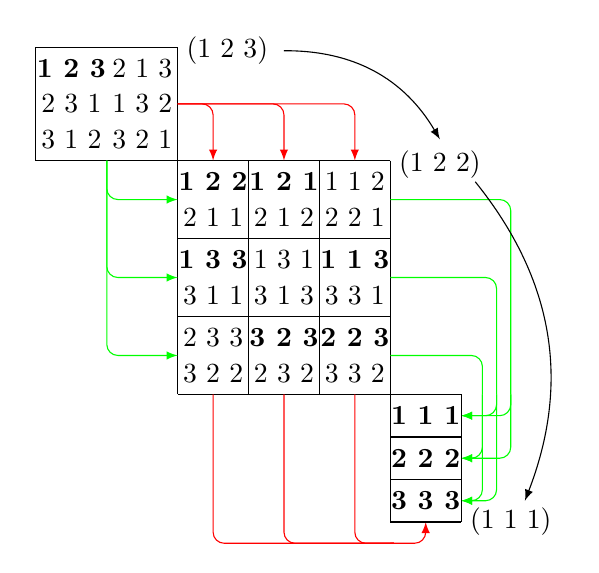
\begin{tikzpicture}[scale = 0.9]
	\tikzstyle{fleche}=[->,>=latex,rounded corners=4pt]
	\node at (2.2,0.25){$\jc$(1 2 3)};
	\node[font = \bfseries] at (0,0){1 2 3};
	\node at (0,-1/2){2 3 1};
	\node at (0,-1){3 1 2};
	\node at (1,0){2 1 3};
	\node at (1,-1/2){1 3 2};
	\node at (1,-1){3 2 1};
	
	
	\draw[black] (-.5,.3) to (1.5, .3);
	\draw[black] (-.5,.3) to (-.5, -1.3);
	\draw[black] (1.5,.3) to (1.5, -4.6);
	\draw[black] (-.5,-1.3) to (4.5, -1.3);
	
	\draw[fleche, red] (1.5,-1/2) -| (2, -1.3);
	\draw[fleche, red] (1.5,-1/2) -| (3, -1.3);
	\draw[fleche, red] (1.5,-1/2) -| (4, -1.3);
	\draw[fleche, green] (.5,-1.3) |- (1.5, -1.85);
	\draw[fleche, green] (.5,-1.3) |- (1.5, -2.95);
	\draw[fleche, green] (.5,-1.3) |- (1.5, -4.05);
	
	\node at (5.2,-1.6+0.25){$\jc$(1 2 2)};
	\draw[->,>=latex, bend left] (3,0.25) to (5.2,-1);
	\node[font = \bfseries] at (2,-1.6){1 2 2};
	\node at (2,-2.1){2 1 1};
	\node[font = \bfseries] at (3,-1.6){1 2 1};
	\node at (3,-2.1){2 1 2};
	\node at (4,-1.6){1 1 2};
	\node at (4,-2.1){2 2 1};
	
	\draw[black] (1.5, -2.4) to (4.5, -2.4);
	
	\node[font = \bfseries] at (2,-2.7){1 3 3};
	\node at (2,-3.2){3 1 1};
	\node at (3,-2.7){1 3 1};
	\node at (3,-3.2){3 1 3};
	\node[font = \bfseries] at (4,-2.7){1 1 3};
	\node at (4,-3.2){3 3 1};
	
	\draw[black] (1.5, -3.5) to (4.5, -3.5);
	
	\node at (2,-3.8){2 3 3};
	\node at (2,-4.3){3 2 2};
	\node[font = \bfseries] at (3,-3.8){3 2 3};
	\node at (3,-4.3){2 3 2};
	\node[font = \bfseries] at (4,-3.8){2 2 3};
	\node at (4,-4.3){3 3 2};
	
	\draw[black] (1.5, -4.6) to (5.5, -4.6);
	\draw[black] (2.5, -1.3) to (2.5, -4.6);
	\draw[black] (3.5, -1.3) to (3.5, -4.6);
	\draw[black] (4.5, -1.3) to (4.5, -6.4);
	
	\draw[rounded corners=4pt, red] (2, -4.6) |- (4.55, -6.7);
	\draw[rounded corners=4pt, red] (3, -4.6) |- (4.55, -6.7);
	\draw[rounded corners=4pt, red] (4, -4.6) |- (4.55, -6.7);
	\draw[fleche, red] (4.5, -6.7) -| (5, -6.4);
	\draw[rounded corners=4pt, green] (4.5, -1.85) -| (6.2, -4.6);
	\draw[fleche, green] (6.2, -4.6) |- (5.5, -4.9);
	\draw[fleche, green] (6.2, -4.6) |- (5.5, -5.5);
	\draw[rounded corners=4pt, green] (4.5, -2.95) -| (6, -4.6);
	\draw[fleche, green] (6, -4.6) |- (5.5, -4.9);
	\draw[fleche, green] (6, -4.6) |- (5.5, -6.1);
	\draw[rounded corners=4pt, green] (4.5, -4.05) -| (5.8, -4.6);
	\draw[fleche, green] (5.8, -4.6) |- (5.5, -6.1);
	\draw[fleche, green] (5.8, -4.6) |- (5.5, -5.5);
	
	\node at (6.2,-6.4){$\jc$(1 1 1)};
	\draw[->,>=latex, bend left] (5.7,-1.6) to (6.4,-6.1);
	\node[font = \bfseries] at (5, -4.9){1 1 1};
	\draw[black] (4.5, -5.2) to (5.5, -5.2);
	\node[font = \bfseries] at (5, -5.5){2 2 2};
	\draw[black] (4.5, -5.8) to (5.5, -5.8);
	\node[font = \bfseries] at (5, -6.1){3 3 3};
	
	\draw[black] (5.5, -4.6) to (5.5, -6.4);
	\draw[black] (4.5, -6.4) to (5.5, -6.4);
	
	\end{tikzpicture}
	\caption[Green relations in $T_3$.]{Green relations in $T_3$. \\ {\small Each block is a $\jc$-class, each line is a $\rc$-class, each column a $\lc$-class and each case an $\hc$-class. The red, green and black arrows represent the $\lc$, $\rc$ and $\jc$-order respectively.}}
\end{figure}\label{fig:green_t3}
			
	The following notations will prove useful, as the study of Green relations is, in part, the study of the maps given by left and right translations in the monoid.
	\begin{notation}\label{not:times}
		Let $h, k$ be elements of $M$ and $S$ be a subset of $M$. We denote by:
		\begin{itemize}
			\item $h\mul{S}$ the application from $S$ to $hS$ defined by $s \mapsto hs$,
			\item $\mul{S}k$ the application from $S$ to $Sk$ defined by $s \mapsto sk$,
			\item ${}_M\stab(S) = \{m \in M \sepp mS = S\}$,
			\item $\stab_M(S) = \{m \in M \sepp Sm = S\}$,
			\item $\fix_S(h, k) = \{s \in S \sepp hsk=s\}$.
		\end{itemize}
	\end{notation}
	
	Using these notations, let us recall Green's Lemma, which is one of the central elements of the theory of Green relations, as it shows that the structure of the relations is actually heavily constrained, making their study practical.
	
	\begin{lemme}[Green's Lemma]\label{lem:green}
		Let $a, a'$ be two elements in the same $\lc$-class and let $\lambda, \lambda'$ such that $\lambda a = a'$ and $\lambda' a' = a$. Then $\lambda\mul{\rc(a)}$ and $\lambda'\mul{\rc(a')}$ are reciprocal bijections. Moreover, for any $\lc$-class $L$ $\lambda\mul{\rc(a)\cap L}$ and $\lambda'\mul{\rc(a')\cap L}$ are reciprocal bijections.
		
		Similarly, if $a, b$ are two elements in the same $\rc$-class and $\rho, \rho'$ are such that $\rho a = b$ and $\rho' b = a$, then $\mul{\lc(a)}\rho$ and $\mul{\lc(b)}\rho'$ are reciprocal bijections. Moreover, for any $\rc$-class $R$ $\mul{\lc(a)\cap R}\rho$ and $\mul{\lc(b)\cap R}\rho'$ are reciprocal bijections.
	\end{lemme}
	
	\begin{figure}[h!]
	\centering
	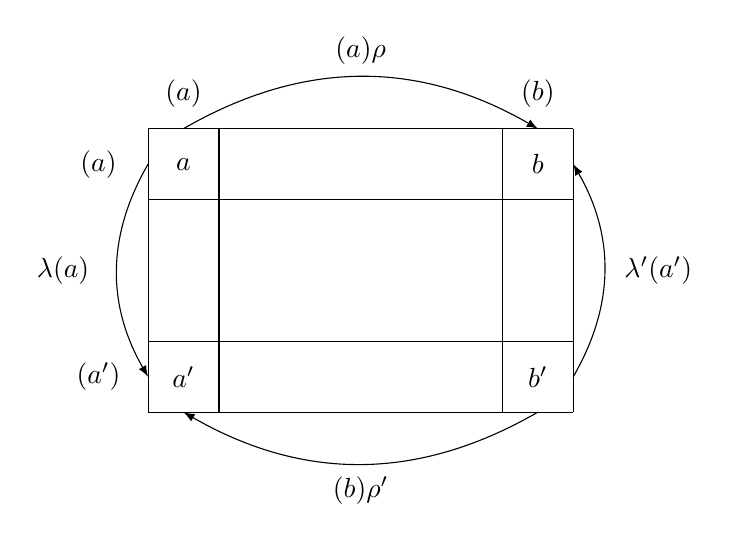
\begin{tikzpicture}[scale = 0.9]
	\tikzstyle{fleche}=[->,>=latex,rounded corners=4pt]
	\node at (0,0){$a'$};
	\node at (0,3){$a$};
	\node at (5,0){$b'$};
	\node at (5,3){$b$};
	\draw (-.5,3.5) -- (-.5, -.5);
	\draw (.5,3.5) -- (.5, -.5);
	\draw (5.5,3.5) -- (5.5, -.5);
	\draw (4.5,3.5) -- (4.5, -.5);
	\draw (-.5,3.5) -- (5.5, 3.5);
	\draw (-.5,2.5) -- (5.5, 2.5);
	\draw (-.5,.5) -- (5.5, .5);
	\draw (-.5,-.5) -- (5.5, -.5);
	
	\draw[->, >=latex, bend right] (-.5,3) to (-.5,0);
	\node at (-1.7, 1.5){$\lambda\mul{\rc(a)}$};
	\draw[->, >=latex, bend right] (5.5,0) to (5.5,3);
	\node at (6.7, 1.5){$\lambda'\mul{\rc(a')}$};
	\draw[->, >=latex, bend left] (0,3.5) to (5,3.5);
	\node at (2.5, 4.6){$\mul{\lc(a)}\rho$};
	\draw[->, >=latex, bend left] (5,-.5) to (0,-.5);
	\node at (2.5, -1.6){$\mul{\lc(b)}\rho'$};
	
	\node at (-1.2, 3){$\rc(a)$};
	\node at (-1.2, 0){$\rc(a')$};
	\node at (0, 4){$\lc(a)$};
	\node at (5, 4){$\lc(b)$};
	
	\end{tikzpicture}
	\caption{Green's Lemma}
\end{figure}
	
	An important consequence of Green's Lemma is that $\jc$-classes can be neatly organized as \emph{eggbox pictures}\footnote{Terminology introduced in \cite{clifford1961algebraic}}: the $\jc$-class can be represented as a rectangular array with the $\lc$-classes as columns, the $\rc$-classes as rows and the $\hc$-classes, the eggs, in the cases, as can be seen in Figure \ref{fig:green_t3}. This level organization is actually what allows for efficient computer representation of monoids and most of their algorithmic exploration. 
	
	\subsubsection{\schu groups}
	
	The Green structure offers a second way of facilitating computer exploration of monoids through groups that arise as stabilizers of some Green classes. These are called the \emph{\schu groups} and -- this a running theme of monoid theory -- allow for a number of monoid theoretic questions to be formulated in terms of groups for which we dispose of an array of efficient algorithms.
	
	\begin{dftn}[\schu groups]\label{def:schu_groups}
		Let $H$ be an $\hc$-class. The set $\{ h\mul{H} \sepp h \in {}_M\stab(H)\}$ equipped with map composition is a subgroup of $\symm(H)$ called the \emph{left \schu group} and denoted by $\Gamma(H)$.
		
		Similarly, $(\{ \mul{H}k \sepp k \in \stab_M(H)\}, \circ)$ is a subgroup of $\symm(H)$ called the \emph{right \schu group} and denoted by $\Gamma'(H)$.
	\end{dftn}

	\begin{lined}
		\begin{ex}\label{ex:schu_as_symm}
			Consider $H = \hc([1\ 3\ 1])$ (the elements of $T_n$ are given in function notation in all examples). We have :
			\[{}_M\stab(H) = \{[1\ 2\ 3], [3\ 2\ 1], [1\ 3\ 3], [3\ 1\ 1], [1\ 1\ 3], [3\ 3\ 1]\}\]
			and subsequently, $\Gamma(H) = \{[1\ 2\ 3]\mul{H}, [3\ 3\ 1]\mul{H}\}$. Notice that, as elements of $\Gamma(H)$, $[3\ 3\ 1]\mul{H} = [3\ 2\ 1]\mul{H}$ and that the only important thing is the permutations induced by the elements of ${}_M\stab(H)$ on $\im H$. Thus, in the case of transformation monoids, the left \schu group of an $\hc$-class $H$ can be represented as a subgroup of $\symm(\im H)$. In the same way, the right \schu groups can be represented as subgroups of $\symm(\ker H)$. This fact is used to represent the \schu groups in Section \ref{sec:Algos}.
		\end{ex}
	\end{lined}

	Our precedent remark on exploiting \schu groups to get efficient algorithms for computational monoid theoretic questions is seconded by the fact that \schu groups do not contain any "superfluous information" in the following sense.
	
	\begin{prop}\label{prop:schu_acts_freely}
		Let $H$ be an $\hc$-class. The natural actions of  $\Gamma(H)$ and $\Gamma'(H)$ on $H$ are free and transitive.
	\end{prop}
	
	We reproduce below a proof for Proposition \ref{prop:schu_acts_freely} from \cite{schu} for the purpose of showcasing the main argument. The argument itself is widely known and we will use it multiple times in the remainder of this paper.
	
	\begin{proof}
		 Two elements $h, h' \in H$ are in the same $\lc$-class so there is some $u \in M$ such that $uh=h'$. By Green's Lemma, this means that $u \in {}_M\stab(H)$, so $\Gamma(H)$ acts transitively on $H$. Suppose that $uh = h$ for some $u\in M$. Since $h, h'$ are also in the same $\rc$ class, there is some $v$ such that $h' = hv$, so $uh'=uhv=hv=h'$ : an element of $\Gamma(H)$ either fixes all points in $H$ or fixes none. The only element of $\Gamma(H)$ that fixes all points (and, consequently, the only one that fixes any point) is the identity and thus the action is free. The same arguments apply for $\Gamma'(H)$.
	\end{proof}
	
	A special case that is interesting to note, and that will be important later, it the case where $H$ is the $\hc$-class of an idempotent :
	
	\begin{dftn}\label{dftn:idem_and_maxgrp}
		An element $e \in M$ is \emph{idempotent} if $e^2=e$. Given an idempotent $e$, the set $G_e = \{x \in M\sepp \exists y \in M, xy=yx=e\}$ is called the \emph{maximal subgroup at $e$}. One can check that $G_e$ is indeed a group and that $G_e = \hc(e)$.
	\end{dftn}

	In that case, $\Gamma(H)$ and $\Gamma'(H)$ can be defined as before, and are canonically isomorphic to $G_e$, simply because $G_e \subset {}_M\stab(H)$ naturally induce a map making it a subgroup of $\Gamma(H)$ and that since $G_e$ acts freely and transitively on $H$, this map must be injective and surjective (and similarly for $\Gamma'(H)$).
	
	\begin{lined}
		\begin{ex}\label{ex:iso_idem}
			Consider, in Example \ref{ex:green_tn}, $e = [1\ 2\ 2]$ and $H = \hc(e)$. $e$ is an idempotent, and, indeed, $H = G_e$ is group : setting $t = [2\ 1\ 1]$, we have $e^2=e, t^2=e$ and $et=te=t$.
			As noted in Example \ref{ex:schu_as_symm} :
			\[\Gamma(H) = \symm(\{1, 2\}), \qquad \Gamma'(H) = \symm(\{\{1\}, \{2,3\}\}).\]
			Note that the canonical isomorphism between $\Gamma(H)$ and $\hc(e)$ is simply given by $g \in \Gamma(H) \mapsto g \cdot e \in H$.
		\end{ex}
	\end{lined}
	
	\subsection{Counting fixed points}\label{sec:fixed}
		Consider the problem of counting the number of elements of the set $\fix_{G}(h, k)$ %$ = \{g \in G \sepp hgk = g\}$ 
	where $G$ is a finite group and $h, k \in G$. 
	If $\fix_{G}(h, k)$ is non-empty, it contains an element $\gamma$ such that $h\gamma k = \gamma$, or equivalently $h = \gamma k\inv \gamma\inv$. So for any $g \in \fix_G(h, k)$ we have:
	\[hgk = g \Leftrightarrow \gamma k\inv \gamma\inv g k = g \Leftrightarrow \gamma\inv g k = k\gamma\inv g.\]
	This means that $g \in \gamma C_G(k)$ where $C_G(k)$ is the centralizer of $k$ in $G$. Because the other inclusion is obvious, we get a description of $|\fix_{G}(h, k)|$: either $h$ and $k\inv$ are conjugated in which case there are $|C_G(k)|$ fixed points, or they are not, and there are no fixed points.
	In the case of a monoid, this reasoning mostly breaks: we crucially used the invertibility property, which monoids lack. The \schu groups seem to be ideal candidates to get back some of this invertibility. 
	In this section we clarify the role of the \schu groups for counting fixed points, how to give meaning to "$h\mul{H}$ and $\mul{H}k$ are in the same conjugacy class", and how to factorize our previous remark over all the $\hc$-classes of the same $\jc$-class.
	
	As the bijections between $\lc$ (and $\rc$) classes will play an major role in the remainder of this section, we introduce the following notations.
	\begin{notation}
		Given $R, R'$ two $\rc$-classes in the same $\jc$-class, we say that $(\lambda, \lambda')$ is a \emph{left Green pair} with respect to $(R, R')$ if:
		\begin{itemize}
			\item $\lambda R = R'$ and $\lambda'R' = R$.
			\item $(\lambda\lambda')\mul{R} = \Id_R$ and $(\lambda'\lambda)\mul{R'} = \Id_{R'}$
		\end{itemize}
		Similarly, given two $\lc$-classes $L, L'$ in the same $\jc$-classes, $(\rho, \rho')$ is a \emph{right Green pair} with respect to $(L, L')$ if:
		\begin{itemize}
			\item $L\rho = L'$ and $L'\rho' = L$.
			\item $\mul{L}(\rho\rho') = \Id_L$ and $\mul{L'}(\rho'\rho) = \Id_{L'}$
		\end{itemize}
	\end{notation}
	
	Using Green pairs, one can transport the problem of counting fixed points in an arbitrary $\hc$-class to a reference $\hc$-class.
	
	\begin{prop}\label{prop:transition}
		Let $H_1, H_2 \subset J$ be two $\hc$-classes contained in the same $\jc$-class. Let $\lambda, \lambda', \rho, \rho'$ such that:
		\begin{itemize}
			\item $(\lambda, \lambda')$ is a left Green pair with respect to $(\rc(H_1), \rc(H_2))$,
			\item $(\rho, \rho')$ is a right Green pair with respect to $(\lc(H_1), \lc(H_2))$.
		\end{itemize}
		Finally, let $(h, k) \in {}_M\stab(\rc(H_2)) \times \stab_M(\lc(H_2))$ and define $(h', k') = (\lambda' h \lambda, \rho k \rho')$. Then the maps $x \mapsto \lambda'x\rho'$ and $x \mapsto \lambda x\rho$ are reciprocal bijections between the sets $\fix_{H_2}(h, k) = \{a \in H_2 \sepp hak = a\}$ and $\fix_{H_1}(h', k')=\{a \in H_1 \sepp h'ak' = a\}$.
	\end{prop}
	
	\begin{proof}
		First notice that Green's Lemma give us the existence of $\lambda, \lambda', \rho, \rho'$ respecting the hypothesis we demand, and also gives that $x \mapsto \lambda'x\rho'$ and $x \mapsto \lambda x\rho$ are reciprocal bijections between $H_1$ and $H_2$.
		Let $a_1$ be an element of $H_1$ and denote by $a_2 = \lambda a_1 \rho$. Then:
		\[ha_2k = a_2 \Leftrightarrow \lambda'ha_2k\rho' = \lambda'a_2\rho' \Leftrightarrow (\lambda' h \lambda)a_1(\rho k \rho') = a_1 \Leftrightarrow h'a_1k' = a_1\]
		so these bijections restrict to $\fix_{H_1}(h', k')$ and $\fix_{H_2}(h, k)$.
	\end{proof}
	
	%\todo{Une image avec le nombre de pts fixes dans chaque H-class}
	
	Keeping in mind our computational goals, transporting the problem of counting fixed points from $H_2$ to $H_1$ is helpful, as for the price of 4 monoid multiplications, we can use a lot of precomputations specific to a particular $\hc$-class, avoiding the repetition of multiple similar computations for each $\hc$-class. 
	
	The question is now to determine the fixed points in a single $\hc$-class, using our previous remark on conjugacy. Let us first clarify the idea of elements of the left and right \schu groups being in the same conjugacy class.
	
	\begin{prop}\label{prop:bij_cano_conj}
		Given and $\hc$-class $H$, $a \in H$ and $g \in \Gamma(H)$, we define $\tau_a(g)$ as the unique element of $\Gamma'(H)$ such that $g \cdot a = a \cdot \tau_a(g)$. Then $\tau_a : \Gamma(H) \longrightarrow \Gamma'(H)$ is an anti-isomorphism\footnote{Note that some authors equip the right \schu group with reversed composition, and thus obtain an isomorphism instead of anti-isomorphism.}. Moreover $\tau_a$ gives rise to a bijection between the conjugacy classes of $\Gamma(H)$ and $\Gamma'(H)$ that is independent of the choice of $a$.
	\end{prop}
	
	\begin{proof}
		The first part is known since \cite{schu}. We want to check that for $a \in H, g \in \Gamma(H)$, the conjugacy class of $\tau_a(g)$ is defined independently of $a$. Take any $a, b \in H$. By definition of $\Gamma(H)$, there exist some $h \in \Gamma(H)$ such that $b = h \cdot a$. So :
		\[b \cdot \tau_a(g) = (h \cdot a) \cdot \tau_a(g) = h \cdot (g \cdot a) = hgh\inv\cdot(h \cdot a) = b \cdot \tau_b(hgh\inv). \]
		Since $\Gamma'(H)$ acts freely, this means that $\tau_a(g) = \tau_b(h)\tau_b(g)\tau_b(h)\inv$ and thus $\tau_a(g)$ is conjugated with $\tau_b(g)$, which proves that the conjugacy class of $\tau_a(g)$ is indeed defined independently of $a$. Finally, as $\tau_a$ is a group morphism, the image are of two conjugated elements are conjugated, meaning that $\tau_a$ does indeed induces bijection between the conjugacy classes of the left and right \schu groups, independently of the choice of $a$.
	\end{proof}

	In the next proposition, we formalize the idea of searching the fixed points as some centralizer, but in the context of a monoid.

	\begin{prop}\label{prop:centralisateur}
		Let $H$ be a $\hc$-class, $a\in H$ and $(h, k) \in {}_M\stab(\rc(H)) \times \stab_M(\lc(H))$. Then
		\[|\fix_H(h, k)| = \left\{\begin{aligned}
		&|C_{\Gamma'(H)}(\mul{H}k)| & & \textrm{ if } \tau_a(h\mul{H})\inv \in \overline{\mul{H}k}\\
		&0 & & \textrm{ otherwise}
		\end{aligned}\right.\]
		where $\overline{\mul{H}k}$ is the conjugacy class of $\mul{H}k$ in $\Gamma'(H)$ and $C_{\Gamma'(H)}(\mul{H}k)$ is the centralizer in $\Gamma'(H)$ of $\mul{H}k$.
	\end{prop}
	
	\begin{proof}
		For simplicity, we commit an abuse of notation by denoting $h\mul{H}$ as $h$ and $\mul{H}k$ as $k$. Let $a$ be any element of $H$. 
		\begin{align*}
		\fix_H(h,k) & = \{b \in H \sepp hbk=b\}\\
		& = \{a \cdot g\sepp g \in \Gamma'(H) \textrm{ and } ha\cdot gk = a\cdot g \}\\
		& = \{a\cdot g\sepp g \in \Gamma'(H) \textrm{ and } a \cdot \tau_a(h)gk = a\cdot g \}\\
		& = \{a\cdot g\sepp g \in \Gamma'(H) \textrm{ and } \tau_a(h)gk = g\}.
		\end{align*}
		The last equality comes from the fact that $\Gamma'(H)$ acts freely so we can simplify the $a$. Suppose that $\fix_H(h, k)$ is non-empty and let $\gamma \in \Gamma'(H)$ such that $\tau_a(h)\gamma k = \gamma$. Then, for any $g \in \Gamma'(H)$ :
		\[\tau_a(h)gk = g \Leftrightarrow g \inv \tau_a(h)gk = e \Leftrightarrow g\inv\gamma k\inv\gamma\inv g k\ = e \Leftrightarrow [\gamma\inv g, k] = e\]
		where $[\cdot,\cdot]$ is the commutation bracket. This means that 
		\[\fix_H(h,k) = \{a \cdot g \sepp g \in \gamma C_{\Gamma'(H)}(k)\}.\]
		Note that because, again, $\Gamma'(H)$ acts freely, $\fix_H(h,k)$ has the same cardinality as $C_{\Gamma'(H)}(k)$ and that, from Proposition \ref{prop:bij_cano_conj} this is independent from the choice of $a$ which proves the result. 
	\end{proof}
	
	\begin{lined}
		\begin{ex}
			Consider $a = [1\ 2\ 2\ 3] \in T_4$ and $H = \hc(a)$. We have $\im a = \{1, 2, 3\}$ and $\ker a = \{\{1\},\{2,3\},\{4\}\}$. Notice that $H$ is not a group since $a^2 = [1\ 2\ 2\ 2] \notin H$. Considering the \schu groups as symmetric groups on the image and kernel common to all elements of $H$ as in Example \ref{ex:schu_as_symm}, we have $\Gamma(H) = \symm(\im a)$ and $\Gamma'(H) = \symm(\ker a)$.
			
			Let us first check for fixed points under the action of $h = [1\ 2\ 3\ 4]$ on the left and $k = [2\ 1\ 1\ 4]$ on the right. Seen as an element of $\Gamma(H)$, $h$ corresponds to $\Id_{\im a}$ and $k$ corresponds to $(\{2, 3\}\ \{1\})$ in $\Gamma'(H)$. Since we have $\tau_a(h) = \Id_{\ker a}$, it follows that $|\fix_H(h,k)| = 0$.
			
			If we now take $h$ to be $[1\ 3\ 2\ 4]$, the corresponding element in $\Gamma(H)$ is $(2\ 3)$ and $\tau_a(h) = (\{2, 3\}\ \{4\})$. Since $(\{2, 3\}\ \{4\})$ and $(\{2, 3\}\ \{1\})$ are conjugated in $\symm(\ker a)$, the set of fixed points is non-empty. Their centralizers have cardinal 2 and one can indeed check that $[2\ 3\ 3\ 1]$ and $[3\ 2\ 2\ 1]$ are the only fixed points in $H$.
		\end{ex}
	\end{lined}

	Putting together the previous results, we get the following Corollary on the cardinality of $\fix_J(h, k)$.
	
	\begin{cor}\label{cor:pt_fix_counting}
		Let $J$ be a $\jc$-class, $a$ any element of $J$ and denote by $H_0 = \hc(a), R_0 = \rc(a), L_0 = \lc(a)$. Let $h, k$ be any elements of $M$. We denote by:
		\begin{itemize}
			\item $(\lambda_R, \lambda'_R)$ a left Green pair with respect to $(R_0, R)$ for each $\rc$-class $R \subset J$,
			\item $(\rho_L, \rho'_L)$ a right Green pair with respect to $(L_0, L)$ for each $\lc$-class $L \subset J$,
			\item $S_{\rc}(h) = \{R \subset J \sepp R \textrm{ is a } \rc\textrm{-class and } hR = R\}$,
			\item $S_{\lc}(k) = \{L \subset J \sepp R \textrm{ is a } \lc\textrm{-class and } Lk = L\}$
		\end{itemize}
		Denoting the set of conjugacy classes of $\Gamma'(H_0)$ as $C$, we further define two vectors:
		\begin{itemize}
			\item $r_J(h) = (|C_{\Gamma'(H)}(g)|\cdot|\{R \in S_{\rc}(h)\sepp \tau_a(\lambda_R' h \lambda_R) \in \bar{g}\}|)_{\bar{g}\in C}$,
			\item $l_J(k) = (|\{L \in S_{\lc}(k)\sepp \rho_L' k \rho_L \in \bar{g}\}|)_{\bar{g}\in C}$. 
		\end{itemize}
		Then $\fix_J(h, k)$ has cardinality the dot product of $r_J(h)$ with $l_J(k)$.
	\end{cor}
	
	
	\section{Modules: character table and Cartan matrix}\label{sec:mod}
	\section{Introduction}

The increasing complexity of source code poses a key challenge to the reliability of large-scale software systems. Software bugs in these systems can lead to safety issues~\cite{bug_safety} for users around the world as well as cause non-negligible financial losses~\cite{bug_loss}. As such, developers have to spend a large amount of time and effort on bug fixing. Consequently, \aprfull (\apr), designed to automatically generate patches to fix software bugs, has attracted wide attention from both academia and industry~\cite{long2016prophet, legoues2012genprog, long2015spr, lou2020can, tufano2018empstudy}. 


To achieve \apr, one popular approach is known as Generate-and-Validate (G\&V)~\cite{qi2015gv, ghanbari2019prapr, lou2020can, le2016hdrepair, legoues2012genprog, wen2018capgen, hua2018sketchfix, martinez2016astor, koyuncu2020fixminder, liu2019tbar, liu2019avatar}, which is typically based on the following pipeline: First, fault localization techniques~\cite{wong2016fl, abreu2007ochiai, zhang2013injecting, papadakis2015metallaxis, li2019deepfl, li2017transforming} are applied to determine the suspicious locations in programs where bugs are likely to exist. Then, the buggy locations are used by the \apr tools to generate a list of patches that replace buggy lines with correct lines. Afterward, each patch is validated against the original test suite to identify any \emph{plausible patches} (i.e., passing all tests in the test suite). Finally, to determine the \emph{correct patches}, developers examine the list of plausible patches to see if any of them can correctly fix the bug. 

Traditional \apr tools can mainly be categorized into heuristic-based~\cite{legoues2012genprog, le2016hdrepair, wen2018capgen}, constraint-based~\cite{mechtaev2016angelix, le2017s3, demacro2014nopol, long2015spr} and \template~\cite{ghanbari2019prapr, hua2018sketchfix, martinez2016astor, liu2019tbar, liu2019avatar}. Among these traditional tools, \template \apr tools~\cite{ghanbari2019prapr, liu2019tbar, benton2020effectiveness} have been able to achieve state-of-the-art results. \Template \apr tools typically leverage pre-defined templates (e.g., adding a nullness check) for bug fixing. However, since these fix templates are typically handcrafted, the number and types of bugs they are able to fix can be limited. 



To address the limitations of traditional \apr, researchers have proposed various \learning \apr tools~\cite{li2020dlfix, chen2018sequencer, jiang2021cure, lutellier2020coconut, zhu2021recoder, ye2022rewardrepair} based on the \nmtfull (\nmt) architecture~\cite{sutskever2014mt} where the input is the buggy code snippets and the goal is to translate the buggy code snippets into a fixed version. To accomplish this, \learning \apr tools require supervised training datasets with pairs of both buggy and fixed code snippets in order to learn how to perform this translation step. These training data are usually obtained by mining historical bug fixes using heuristics/keywords~\cite{dallmeier2007benchmark}, which can be imprecise for identifying bug-fixing commits; even the actual bug-fixing commits can include irrelevant code changes, leading to further pollution in the dataset~\cite{xia2022alpharepair}.
% 
Moreover, it can be hard for such \apr tools to generalize and fix bug types unseen during training. 



To better leverage recent advances in \plmfull{s} (\plm{s}), researchers~\cite{xia2022alpharepair, xia2023repairstudy, kolak2022patch, prenner2021codexws} have directly applied \plm{s} to generate patches without bug-fixing datasets. These \llm-based \apr tools work by either directly generating a complete code function~\cite{prenner2021codexws, xia2023repairstudy} or predict/infill the correct code snippet given its surrounding context~\cite{xia2022alpharepair, xia2023repairstudy}. By directly using \llm{s} that are pre-trained on billions of open-source code snippets, \llm-based \apr tools can achieve state-of-the-art performance on many repair datasets~\cite{xia2022alpharepair}. 


% 
%
%

Traditional \apr tools have long used the insight of the \emph{plastic surgery hypothesis}~\cite{barr2014plastic} where it states that the code ingredients to fix a bug already exist within the same project. Traditional \apr tools have manually designed pattern-~\cite{ghanbari2019prapr, saha2017elixir} or heuristic-based~\cite{jiang2018simfix, legoues2012genprog} approaches to finding and using such relevant code ingredients to generate fixes for bugs. However, the plastic surgery hypothesis has been largely ignored in \llm-based \apr. In fact, \llm provides a unique opportunity to fully automate the plastic surgery hypothesis idea via fine-tuning (learning project-specific information via model updates from the buggy project) and prompting (directly providing relevant code ingredients to the model), and make it directly applicable to different languages (since the \llm{s} are typically multi-lingual).%
Moreover, despite the intensive manual efforts involved, traditional \apr tools still cannot fully leverage project-specific information due to large search space for leveraging/composing existing code ingredients. In contrast, the project-specific information can effectively leveraged by \llm{s} due to their power in code understanding/vectorization, e.g., even partial/imprecise information may still guide \llm{s} in correct patch generation!
 To this end, we ask the question: \emph{How useful is the plastic surgery hypothesis in the era of \plm{s}}?








\mypara{Our Work.} To answer the question, we present \ourtech{\xspace} -- a \llm-based approach that automatically utilizes the plastic surgery hypothesis by systematically combining multiple fine-tuning and prompting strategies for \apr. \ourtech fine-tunes \plm{s} using two novel domain-specific training strategies: \textbf{\epfinetune} -- we fine-tune using the original buggy project by aggressively masking out a high percentage of tokens, which allows \plm to learn project-specific code tokens and programming styles; and \textbf{\rofinetune} -- which only masks out a single continuous code sequence per training sample, allowing the model to get used to the final \csapr task of predicting a single continuous code sequence. Furthermore, we directly leverage the ability for \plm{s} to understand natural language instructions and introduce a novel prompting strategy, \textbf{\idprompting}, which uses information retrieval and static analysis to obtain a list of relevant identifiers for the buggy lines. While such relevant identifiers are critical for fixing some difficult bugs, they may not be seen by the \llm during inference due to limited context window size. Through the use of prompting, we directly tell the model to use these extracted identifiers (relevant code ingredients) to generate the correct code. Finally, to perform repair, we combine all four model variants (including the base model, both fine-tuned models and the base model with prompting) for the final repair.





While our insight of leveraging the plastic surgery hypothesis for \llm-based \apr is generalizable across different types of \plm{s}, to implement \ourtech, we choose a recent \plm{\xspace}, \ctfive~\cite{wang2021codet5}, which is pre-trained on millions of open-source code snippets. \ctfive is an encoder-decoder model trained using \mspfull (\msp) objective where a percentage of tokens are masked out and each continuous masked token sequence is referred to as a masked span. Also, although we only extract relevant identifiers from the current buggy project (since this paper focuses on the plastic surgery hypothesis), our work can be easily extended to obtain other code information (such as relevant statements or functions) from other sources, such as  the massive pre-training corpora~\cite{husain2020codesearchnet} or historical bug-fixing datasets~\cite{jiang2019infer}, which can provide more coding knowledge for \llm{s}. Besides, although we mainly focus on using traditional string comparison algorithms for information retrieval in this paper, these techniques can be easily replaced by other frequency-based retrieval~\cite{robertson2009probabilistic} and neural search (or embedding-based search)~\cite{reimers2019sentence}.
  In summary, this paper makes the following contributions:


%


\begin{itemize}[noitemsep, leftmargin=*, topsep=0pt]
    \item \textbf{Dimension.} This paper is the first to revisit the important plastic surgery hypothesis in the era of \llm{s}. It opens up a new dimension for \llm-based \apr to incorporate previously neglected information from the buggy project itself to boost \apr performance. Furthermore, it demonstrates the promising future of retrieval-based prompting for modern \llm-based \apr.
    \item \textbf{Implementation.} We implement \ourtech based on the recent \ctfive model. We augment the model using two novel fine-tuning strategies: \epfinetune and \rofinetune, along with a novel prompting strategy based on information retrieval and static analysis: \idprompting. We combine the patches generated by all four models together and perform patch ranking to speed up \apr.% 
    \item \textbf{Evaluation Study.} We conduct an extensive evaluation against state-of-the-art \apr tools. On the widely studied \dfj 1.2 and 2.0 datasets~\cite{just2014dfj}, \ourtech is able to achieve the new state-of-the-art results of 89 and 44 correct bug fixes (15 and 8 more than best baseline) respectively.  Furthermore, we perform a broad ablation study to justify our design. \ourtech demonstrates for the first time that the plastic surgery hypothesis can substantially boost \llm-based \apr and advance state-of-the-art \apr, while being fully automated and general. Moreover, even partial/imprecise code ingredients may still effectively guide \llm{s} for \apr!
\end{itemize}



	\subsection{On modules}\label{sub:modules}
	
\usetikzlibrary{shapes, shapes.misc, backgrounds}


\tikzset{%
	on layer/.code={
		\pgfonlayer{#1}\begingroup
		\aftergroup\endpgfonlayer
		\aftergroup\endgroup
}}

\newlength{\ModuleDiagramSymbolSize}
\setlength{\ModuleDiagramSymbolSize}{.2ex}
\tikzset{
	really densely dotted/.style={line cap=round, dash pattern=on 0pt off 2\pgflinewidth},
	module diagram symbol size/.style={
		generator/.style={shape=circle, fill, outer sep=0, inner sep=#1},
		relation/.style={shape=diamond, fill, outer sep=0, inner sep=#1},
		syzygy/.style={shape=cross out, draw, outer sep=0, inner sep=#1}
	},
	every module diagram/.style={
		module diagram symbol size=.2ex,
		line cap=round,
	},
	module diagram/.style={
		every module diagram,
		every picture
	}
}

\newcommand{\Chains}[3][]{
	\node[#1, generator, at=(#2), label={[#1]below:#3}] (G) {};
	\begin{scope}[#1]
		\fill[opacity=0.2] (#2) |- (inf) |- cycle;
		\draw[] (inf -| G) -- (G) -- (G -| inf);
	\end{scope}

}

\NewDocumentCommand{\CochainsAbsolute}{
	s
	O{} % style
	m % node  the simplex grade
	O{} % style for the label
	m % label
	O{below left} % positioning of the label
}{
	\begin{scope}[#2]
		\IfBooleanTF{#1}{
				\coordinate[at=(#3), label={[#2,#4]#6:#5}] (S);
				\coordinate[at=(#3 |- inf)] (R1);
				\coordinate[at=(#3 -| inf)] (R2);
				\coordinate[at=(inf)] (G);
		}{
			\node[syzygy, at=(#3), label={[#2,#4]#6:#5}] (S) {};
			\node[relation, at=(#3 |- inf)] (R1) {};
			\node[relation, at=(#3 -| inf)] (R2) {};
			\node[generator, at=(inf), opacity=.5] (G) {};
		}
		\fill[opacity=0.2] (S.center) |- (inf) |- cycle;
		\IfBooleanTF{#1}{
			\draw (inf -| #3) -- (S) -- (#3 -| inf);
		}{
			\draw
				(pinf -| #3) -- (S) -- (#3 -| pinf)
				(qinf -| #3) -- (R1) -- (G) -- (R2) -- (#3 -| qinf);
			\draw[every picture, really densely dotted]
				(pinf -| #3) -- (qinf -| #3)
				(pinf |- #3) -- (qinf |- #3);
		}
%	\end{scope}
}

\NewDocumentCommand{\CochainsRelative}{%
	s
	O{} % style
	m % name of the node of the simplex
	O{} % style for the labels
	m % label at the simplex grade
	O{above right} % positioning of the label of the simplex grade
	O{} % label at the first generator
	O{} % label at the second generator
}{
	\begin{scope}[#2]
		\IfBooleanTF{#1}{
			\coordinate[at=(#3 |- inf), label={[#4]above:#7}] (G1);
			\coordinate[at=(#3 -| inf), label={[#4]right:#8}] (G2);
			\coordinate[at=(#3), label={[#4]#6:#5}] (R);
		}{
			\node[generator, at=(#3 |- inf), label={[#4]above:#7}] (G1) {};
			\node[generator, at=(#3 -| inf), label={[#4]right:#8}] (G2) {};
			\node[relation, at=(#3), label={[#4]#6:#5}] (R) {};
		}
		\fill[opacity=0.2] (#3) |- (P |- inf) |- (P -| inf) |- (#3);
			\IfBooleanTF{#1}{
				\draw (#3 |- inf) -- (R) -- (#3 -| inf);
			}{
				\draw
					(#3 |- qinf) -- (G1) -- (P |- inf)
					(#3 -| qinf) -- (G2) -- (P -| inf)
					(#3 |- pinf) -- (R) -- (#3 -| pinf);
				\draw[really densely dotted]
					(#3 |- pinf) -- (#3 |- qinf)
					(#3 -| pinf) -- (#3 -| qinf);
			}
	\end{scope}
}

\newcommand{\infinityCoordinate}{4,4}
\newcommand{\coordinates}{
	\coordinate (inf) at (\infinityCoordinate);
	\coordinate (pinf) at ($(inf)-(0.75,0.75)$);
	\coordinate (qinf) at ($(inf)-(0.25,0.25)$);
	\coordinate (O) at (0,0);
	\coordinate (P) at (-0.5,-0.5);
}

\ProvideDocumentCommand{\DrawGrid}{O{0} D(){0.5} m O{0} D(){0.5} m}{
	\begin{scope}[on background layer]
		\foreach \i in {#1, #2, ..., #3}{
			\foreach \j in {#4, #5, ..., #6}{
				\fill[gray] (\i, \j) circle (0.3pt);
			}
		}
	\end{scope}
}

\newcommand{\AxesHomology}{
	\coordinates
	\begin{scope}[]
		\draw[->] (-0.75,0) -- (O -| inf);
		\draw[->] (0,-0.75) -- (O |- inf);
	\end{scope}
}
\NewDocumentCommand{\AxesCohomology}{
	s % without star, draw the 'finitized' version.
}{
	\coordinates
	\begin{scope}[]
		\IfBooleanTF{#1}{
			\draw[<-, shorten <=-8] (0,0) -- (O -| inf);
			\draw[<-, shorten <=-8] (0,0) -- (O |- inf);
		}{
			\draw[<-, shorten <=-8] (0,0) -- (O -| pinf);
			\draw[<-, shorten <=-8] (0,0) -- (O |- pinf);
			\draw[really densely dotted]  (O -| pinf) -- (O -| qinf);
			\draw[really densely dotted] (O |- pinf) -- (O |- qinf);
			\draw          (O -| qinf) -- (O -| inf);
			\draw          (O |- qinf) -- (O |- inf);
		}
	\end{scope}
}


\newcommand{\FreeModule}[3][]{
	\begin{scope}[#1]
		\node[#3, at=(#2)] {};
		\coordinate[at=(#2)] (n) {};
		\fill[opacity=.25] (#2) rectangle (inf);
		\draw (n) -- (n |- inf) (n) -- (n -| inf);
	\end{scope}
}

\newcommand{\InjectiveModule}[2][]{
	\path (#2) coordinate (n);
	\fill[#1, opacity=.25] (n) rectangle (P);
	\draw[#1] (n) -- (n |- P) (n) -- (n -| P);
}

	
	\subsection{On characters}\label{sub:char}
	One of the major features of the finite group representation theory is the fact that all the information on a representation can be summarized in its \emph{character}. This (partially) carries over to monoid representation theory, as we shall see in this section where we reformulate the results of the previous section in terms of characters.

\begin{dftn}
	If $V$ is a finite dimension $\kbf M$-module, its \emph{character} is the map from $M$ to $\kbf$ defined by $\chi_{\kbf M}^V : m \longmapsto \tr(v \mapsto m \cdot v)$.
\end{dftn}

We recall the following well know facts about characters.  Proofs for fact 2 and 3 are respectively (ii) and (iii) of \cite[Proposition 7.12]{steinberg2016representation}\footnote{Note that for Fact 3, our reference deals only with the case $M = M'$, but the proof is the same.}.

\begin{prop}\label{prop:facts_on_char}
	\begin{enumerate}
		\item Let $V$ be a $\kbf M$-module. We have $\chi_{\kbf M}^V = \chi_{\kbf M^{op}}^{V^*}$.
		\item Consider the short exact sequence of $\kbf M$-modules :
		\[0 \longrightarrow A \longrightarrow B \longrightarrow B/A \longrightarrow 0.\]
		Then $\chi_{\kbf M}^{B/A} = \chi_{\kbf M}^B - \chi_{\kbf M}^A$.
		\item Consider $M, M'$ two finite monoids, $V$ a $\kbf M$-module and $W$ a $\kbf M'^{op}$-module. Then $\chi_{\kbf M \otimes \kbf M'}^{V \otimes W} = \chi_{\kbf M}^{V} \chi_{\kbf M'}^{W}$.
	\end{enumerate}
\end{prop}

The previous properties are simply extensions of similar properties on groups, and their proof is similar. From groups, we also keep in the case of monoids the linear independence of irreducible characters (see \cite[Theorem 7.7]{steinberg2016representation} for reference):

\begin{prop}\label{prop:char_libres}
	The irreducible characters $\{\chi_{\kbf M}^S \sepp S \textrm{ is a simple } \kbf M-\module\}$ are linearly independent as $\kbf$ valued functions.
\end{prop}

This, together with the second point in the Proposition \ref{prop:facts_on_char}, has a nice consequence. As we are interested in finite dimensional module over finite monoids, those modules have a composition series. Say that a $\kbf M$-module $V$, has $S$ as a composition factor with multiplicity $[V:S]$ for any simple $\kbf M$-module $S$. Then:
\[\chi_{\kbf M}^V = \sum_S [V:S]\chi_{\kbf M}^S.\]
In that way, since characters of the simple modules are linearly independent, the character of a module can be seen as a record of its composition factors.

The question of where to compute characters is worth asking: in the case of groups, one needs only to compute the character for a transversal of conjugacy classes to get its value everywhere. The case of monoids was described for the first time by McAlister in \cite{mcalister1972characters}. 

\begin{dftn}\label{def:conj}
	We say that two elements $m, m'$ in $M$ are in the same \emph{generalized conjugacy class} or \emph{character equivalency class} if for every $\kbf M$-module $V$, $\chi_M^V(m) = \chi_M^V(m')$. We note $C_M$ the set of generalized conjugacy classes.
\end{dftn}

\begin{prop}(\cite[Proposition 2.5]{mcalister1972characters})\label{prop:char_equiv}
	Let $\mathcal{E} = \{e_1, \dots, e_n\}$ be idempotent representatives of the regular $\jc$-classes of $M$ and for each $e_i$ let $\mathcal{C}_i = \{c_{i,1}, \dots, c_{i,m_i}\}$ be representatives of the conjugacy classes of $G_{e_i}$. Then the set $\mathcal{C}_M = \bigcup_{e_i \in \mathcal{E}} \mathcal{C}_i$ is a set of representatives of character equivalency classes of $M$.
\end{prop}

We can now recall the definition of the character table of a monoid.

\begin{dftn}
	Let $\irr_M$ be the set of isomorphism classes of simple $\kbf M$-modules and $C_M$ as in definition \ref{def:conj}.
	The \emph{character table} of $M$ over $\kbf$ is the (square) matrix defined by :
	\[X(M) = (\chi_{\kbf M}^V(m))_{V \in \irr_M, m \in C_M}.\]
	Moreover, if $e \in M$ is an idempotent, we define $X_e(M)$ as the matrix obtained by extracting from $X(M)$ only the lines corresponding to simple modules with apex $e$.
\end{dftn}

Finally, we can apply the language of characters to Proposition \ref{prop:quotient_semisimple}, which yield a formula for computing the character table of $M$ over $\kbf$ given the character tables of the groups $G_e$ over $k$.

\begin{prop}\label{prop:formula_char}
	Let $e \in M$ be an idempotent, $G_e$ be the maximal subgroup at $e$. 
	We have the formula for $X_e(M)$ : 
	\[X_e(M) = {}^tX(G_e)\inv \cdot \left(\chi_{\kbf M \otimes \kbf G_e^{op}}^{\kbf\lc(e)}(m, g) - \chi_{\kbf M \otimes \kbf G_e^{op}}^{N_e(\kbf\lc(e))}(m, g)\right)_{g \in C_{G_e}, m \in C_M}\]
	where the dot is the matrix product.
\end{prop}

\begin{proof}
	First, we have, because of Proposition \ref{prop:facts_on_char}-2, we have:
	\[\chi_{\kbf M \otimes \kbf G_e^{op}}^{\kbf\lc(e)/N_e(\kbf\lc(e))} = 
	\chi_{\kbf M \otimes \kbf G_e^{op}}^{\kbf\lc(e)}(m, g) - \chi_{\kbf M \otimes \kbf G_e^{op}}^{N_e(\kbf\lc(e))}(m, g)\]
	Then, from Proposition \ref{prop:quotient_semisimple}, we know that:
	\[\begin{aligned}
		\chi_{\kbf M \otimes \kbf G_e^{op}}^{\kbf\lc(e)/N_e(\kbf\lc(e))}(m, g) 
		& = \chi_{\kbf M \otimes \kbf G_e^{op}}^{\bigoplus_{V \in \irr_e} V^{\#} \otimes V^*}\\
		& = \sum_{V\in\irr_e} \chi_{\kbf M \otimes \kbf G_e^{op}}^{V^{\#} \otimes V^*}\\
		& = \sum_{V\in\irr_e} \chi_{\kbf M}^{V^{\#}}(m)\chi_{\kbf G_e}^V(g)\\
	\end{aligned}
	\]
	This last sum is clearly the dot product between the column of $X(G_e)$ indexed by $g$ and the column of $X_e(M)$ indexed by $m$. That is, the coefficient in position $(g, m)$ of $\chi_{M-G_e}^{\lc(e)/\rad(\lc(e))}$ is equal to the coefficient in position $(g, m)$ of ${}^tX(G_e)\cdot X_e(M)$, which, together with Proposition \ref{prop:facts_on_char}(ii), proves the equality.
\end{proof}
	
 	\subsection{One step beyond: The Cartan matrix}
	We are, at last, in measure to state the formula from Thiéry for the Cartan Matrix. Without getting into the specific details, the Cartan matrix can be seen as measure of how "not semi-simple" the algebra of the monoid is. 
We use a non standard definition of the Cartan matrix, first given in \cite[Definition 2.6]{Thiery.CartanMatrixMonoid}. A formal proof that this is equivalent to the usual definition can be found in \cite[Corolary 7.28]{steinberg2016representation}.

\begin{dftn}
	Let $\{S_1, \dots, S_n\}$ be a set of representatives of the isomorphism classes of simple $\kbf M$-modules. The simple $\kbf M \otimes \kbf M^{op}$ modules are the $S_i \otimes S_j^*$ for all $i, j \in \intint{1, n}$. Denote by $[\kbf M : S_i \otimes S_j^*]$ the multiplicity of $S_i \otimes S_j^*$ as a composition factor of $\kbf M$.
	
	The Cartan matrix of $\kbf M$ is defined by:
	\[C(\kbf M) = ([\kbf M : S_i \otimes S_j^*])_{i, j}\] 
\end{dftn}

In other words, the Cartan matrix is a recording of the multiplicities of the composition factors of $\kbf M$ as a $\kbf M \otimes \kbf M^{op}$ module. But so is its character! The difference being that the character of $\kbf M$ as it is computed is expressed in the basis of the character equivalency classes of $M \times M^{op}$ while the Cartan matrix is expressed directly in the basis of the simple modules. Since the basis change between the two is precisely given by the character table and hence, we have the Thiéry's Formula for the Cartan matrix.

\begin{prop}\label{prop:formule_cartan}
	The Cartan matrix is given by the formula:
	\[C(\kbf M) = {}^tX_M\inv B X_M\inv\]
	where $B = (|\{s \in M \sepp msm'\}|)_{m,m' \in C_M}$
\end{prop}
	
	\section{Some explicit computations}\label{sec:Algos}
	\section{Introduction}

The increasing complexity of source code poses a key challenge to the reliability of large-scale software systems. Software bugs in these systems can lead to safety issues~\cite{bug_safety} for users around the world as well as cause non-negligible financial losses~\cite{bug_loss}. As such, developers have to spend a large amount of time and effort on bug fixing. Consequently, \aprfull (\apr), designed to automatically generate patches to fix software bugs, has attracted wide attention from both academia and industry~\cite{long2016prophet, legoues2012genprog, long2015spr, lou2020can, tufano2018empstudy}. 


To achieve \apr, one popular approach is known as Generate-and-Validate (G\&V)~\cite{qi2015gv, ghanbari2019prapr, lou2020can, le2016hdrepair, legoues2012genprog, wen2018capgen, hua2018sketchfix, martinez2016astor, koyuncu2020fixminder, liu2019tbar, liu2019avatar}, which is typically based on the following pipeline: First, fault localization techniques~\cite{wong2016fl, abreu2007ochiai, zhang2013injecting, papadakis2015metallaxis, li2019deepfl, li2017transforming} are applied to determine the suspicious locations in programs where bugs are likely to exist. Then, the buggy locations are used by the \apr tools to generate a list of patches that replace buggy lines with correct lines. Afterward, each patch is validated against the original test suite to identify any \emph{plausible patches} (i.e., passing all tests in the test suite). Finally, to determine the \emph{correct patches}, developers examine the list of plausible patches to see if any of them can correctly fix the bug. 

Traditional \apr tools can mainly be categorized into heuristic-based~\cite{legoues2012genprog, le2016hdrepair, wen2018capgen}, constraint-based~\cite{mechtaev2016angelix, le2017s3, demacro2014nopol, long2015spr} and \template~\cite{ghanbari2019prapr, hua2018sketchfix, martinez2016astor, liu2019tbar, liu2019avatar}. Among these traditional tools, \template \apr tools~\cite{ghanbari2019prapr, liu2019tbar, benton2020effectiveness} have been able to achieve state-of-the-art results. \Template \apr tools typically leverage pre-defined templates (e.g., adding a nullness check) for bug fixing. However, since these fix templates are typically handcrafted, the number and types of bugs they are able to fix can be limited. 



To address the limitations of traditional \apr, researchers have proposed various \learning \apr tools~\cite{li2020dlfix, chen2018sequencer, jiang2021cure, lutellier2020coconut, zhu2021recoder, ye2022rewardrepair} based on the \nmtfull (\nmt) architecture~\cite{sutskever2014mt} where the input is the buggy code snippets and the goal is to translate the buggy code snippets into a fixed version. To accomplish this, \learning \apr tools require supervised training datasets with pairs of both buggy and fixed code snippets in order to learn how to perform this translation step. These training data are usually obtained by mining historical bug fixes using heuristics/keywords~\cite{dallmeier2007benchmark}, which can be imprecise for identifying bug-fixing commits; even the actual bug-fixing commits can include irrelevant code changes, leading to further pollution in the dataset~\cite{xia2022alpharepair}.
% 
Moreover, it can be hard for such \apr tools to generalize and fix bug types unseen during training. 



To better leverage recent advances in \plmfull{s} (\plm{s}), researchers~\cite{xia2022alpharepair, xia2023repairstudy, kolak2022patch, prenner2021codexws} have directly applied \plm{s} to generate patches without bug-fixing datasets. These \llm-based \apr tools work by either directly generating a complete code function~\cite{prenner2021codexws, xia2023repairstudy} or predict/infill the correct code snippet given its surrounding context~\cite{xia2022alpharepair, xia2023repairstudy}. By directly using \llm{s} that are pre-trained on billions of open-source code snippets, \llm-based \apr tools can achieve state-of-the-art performance on many repair datasets~\cite{xia2022alpharepair}. 


% 
%
%

Traditional \apr tools have long used the insight of the \emph{plastic surgery hypothesis}~\cite{barr2014plastic} where it states that the code ingredients to fix a bug already exist within the same project. Traditional \apr tools have manually designed pattern-~\cite{ghanbari2019prapr, saha2017elixir} or heuristic-based~\cite{jiang2018simfix, legoues2012genprog} approaches to finding and using such relevant code ingredients to generate fixes for bugs. However, the plastic surgery hypothesis has been largely ignored in \llm-based \apr. In fact, \llm provides a unique opportunity to fully automate the plastic surgery hypothesis idea via fine-tuning (learning project-specific information via model updates from the buggy project) and prompting (directly providing relevant code ingredients to the model), and make it directly applicable to different languages (since the \llm{s} are typically multi-lingual).%
Moreover, despite the intensive manual efforts involved, traditional \apr tools still cannot fully leverage project-specific information due to large search space for leveraging/composing existing code ingredients. In contrast, the project-specific information can effectively leveraged by \llm{s} due to their power in code understanding/vectorization, e.g., even partial/imprecise information may still guide \llm{s} in correct patch generation!
 To this end, we ask the question: \emph{How useful is the plastic surgery hypothesis in the era of \plm{s}}?








\mypara{Our Work.} To answer the question, we present \ourtech{\xspace} -- a \llm-based approach that automatically utilizes the plastic surgery hypothesis by systematically combining multiple fine-tuning and prompting strategies for \apr. \ourtech fine-tunes \plm{s} using two novel domain-specific training strategies: \textbf{\epfinetune} -- we fine-tune using the original buggy project by aggressively masking out a high percentage of tokens, which allows \plm to learn project-specific code tokens and programming styles; and \textbf{\rofinetune} -- which only masks out a single continuous code sequence per training sample, allowing the model to get used to the final \csapr task of predicting a single continuous code sequence. Furthermore, we directly leverage the ability for \plm{s} to understand natural language instructions and introduce a novel prompting strategy, \textbf{\idprompting}, which uses information retrieval and static analysis to obtain a list of relevant identifiers for the buggy lines. While such relevant identifiers are critical for fixing some difficult bugs, they may not be seen by the \llm during inference due to limited context window size. Through the use of prompting, we directly tell the model to use these extracted identifiers (relevant code ingredients) to generate the correct code. Finally, to perform repair, we combine all four model variants (including the base model, both fine-tuned models and the base model with prompting) for the final repair.





While our insight of leveraging the plastic surgery hypothesis for \llm-based \apr is generalizable across different types of \plm{s}, to implement \ourtech, we choose a recent \plm{\xspace}, \ctfive~\cite{wang2021codet5}, which is pre-trained on millions of open-source code snippets. \ctfive is an encoder-decoder model trained using \mspfull (\msp) objective where a percentage of tokens are masked out and each continuous masked token sequence is referred to as a masked span. Also, although we only extract relevant identifiers from the current buggy project (since this paper focuses on the plastic surgery hypothesis), our work can be easily extended to obtain other code information (such as relevant statements or functions) from other sources, such as  the massive pre-training corpora~\cite{husain2020codesearchnet} or historical bug-fixing datasets~\cite{jiang2019infer}, which can provide more coding knowledge for \llm{s}. Besides, although we mainly focus on using traditional string comparison algorithms for information retrieval in this paper, these techniques can be easily replaced by other frequency-based retrieval~\cite{robertson2009probabilistic} and neural search (or embedding-based search)~\cite{reimers2019sentence}.
  In summary, this paper makes the following contributions:


%


\begin{itemize}[noitemsep, leftmargin=*, topsep=0pt]
    \item \textbf{Dimension.} This paper is the first to revisit the important plastic surgery hypothesis in the era of \llm{s}. It opens up a new dimension for \llm-based \apr to incorporate previously neglected information from the buggy project itself to boost \apr performance. Furthermore, it demonstrates the promising future of retrieval-based prompting for modern \llm-based \apr.
    \item \textbf{Implementation.} We implement \ourtech based on the recent \ctfive model. We augment the model using two novel fine-tuning strategies: \epfinetune and \rofinetune, along with a novel prompting strategy based on information retrieval and static analysis: \idprompting. We combine the patches generated by all four models together and perform patch ranking to speed up \apr.% 
    \item \textbf{Evaluation Study.} We conduct an extensive evaluation against state-of-the-art \apr tools. On the widely studied \dfj 1.2 and 2.0 datasets~\cite{just2014dfj}, \ourtech is able to achieve the new state-of-the-art results of 89 and 44 correct bug fixes (15 and 8 more than best baseline) respectively.  Furthermore, we perform a broad ablation study to justify our design. \ourtech demonstrates for the first time that the plastic surgery hypothesis can substantially boost \llm-based \apr and advance state-of-the-art \apr, while being fully automated and general. Moreover, even partial/imprecise code ingredients may still effectively guide \llm{s} for \apr!
\end{itemize}


	
	\subsection{Computational hypotheses}\label{sub:hypo}
	In this section we discuss the computational hypotheses necessary for the algorithms in the next section. 
This section is based on the work \cite{east2019computing} in which East, Egry-Nagy, Mitchell and Péresse provide efficient algorithms for all basic computational questions on finite semigroups (which include monoids). Although we limit our scope to the case of transformation monoids, methods described \cite{east2019computing} allow the algorithms described below to be applied to other interesting classes of monoids. Moreover, they can theoretically be applied to any finite monoid using a Cayley embedding in a full transformation monoid. In general however, this is very inefficient and not feasible in practice.

Following the authors of \cite{east2019computing}, we make the following fundamental assumptions that we can compute:  
\begin{itemize}
	\item Assumption I : a product of two elements of the monoid.
	\item Assumption II : the image and kernel of a transformation (note that we do not explicitly use this assumption, but that it is necessary for the algorithms of \cite{east2019computing} that we do use).
	\item Assumption III : Green pairs.
	\item Assumption IV : Given $h \in {}_M\stab(H)$ compute the corresponding element in $\Gamma(H)$ (understood as a permutation group of the image common to all elements of $H$ as seen in Example \ref{ex:schu_as_symm}), and similarly on the right.
\end{itemize}

Not only do we directly need to be able to do these computations for our own algorithm, but they are also prerequisite for the algorithms from \cite{east2019computing}. As such, we refer to the top of Section 5.2 of \cite{east2019computing} on how to realize these computations in the case of transformation monoids.

We, again, refer to \cite{east2019computing} for the specific algorithms meeting our computational prerequisites.
\begin{itemize}
	\item Computing the \schu groups: \cite[Algorithm 4]{east2019computing}
	\item Checking membership of an element in a Green class: \cite[Algorithms 7 \& 8]{east2019computing}.
	\item Finding idempotents: \cite[Algorithm 10]{east2019computing}. This algorithm also allows for finding the regular $\jc$-classes.
	\item Decomposing the monoid in $\rc, \lc$ and $\jc$-classes : \cite[Algorithm 11]{east2019computing} and its discussion. Note that by storing this decomposition, we can, given an element of the monoid, find the classes that contain it.
	\item Obtaining a representative of a Green class: this is given by the data structure representing the Green classes described at the top of \cite[Section 5.4]{east2019computing}.
\end{itemize}

Finally, we require the following points that, although they are not described in \cite{east2019computing}, are easily obtained from it.

\begin{itemize}
	\item Computing a set $C_M$ of character equivalency representatives: given Proposition \ref{prop:char_equiv}, this can be done in four steps:
	\begin{enumerate}
		\item compute a set $\mathcal{E}$ of idempotent representatives of the regular $\jc$-classes,
		\item compute $\Gamma(\hc(e))$ for each $e \in \mathcal{E}$,
		\item compute a set $C_e$ of representatives of the conjugacy classes of $\Gamma(\hc(e))$ for each $e \in \mathcal{E}$, using for instance the procedure described in \cite{hulpke2000conjugacy},
		\item for each $e \in \mathcal{E}$ and $c \in C_e$ compute the corresponding element of $\hc(e)$ as in Example \ref{ex:iso_idem}. 
	\end{enumerate}
	\item Computing $\tau_a$ as in Proposition \ref{prop:bij_cano_conj} :  given $g \in \Gamma(H)$, $\tau_a(g)$ is simply, seen as an element of $\symm(\ker a)$ :
	\[a\inv\{i\} \mapsto (g\cdot a)\inv\{g\cdot a(i)\},\]
	which can be computed in $O(n)$. Note that this is a special case of the application described in \cite[Proposition 3.11 (a)]{east2019computing}
	\item Testing that two elements $g, g'$ in $\Gamma'(\hc(a))$ are conjugated : $\Gamma'(H)$ is represented as a subgroup of $\symm(\ker a)$ and known procedures, such as the one described in \cite{butler1994inductive}, can be used.
	\item Computing the cardinality of a conjugacy class of a \schu group: for instance, the computer algebra system GAP uses the method described in \cite{hulpke2000conjugacy}.
\end{itemize}
	
	\subsection{Combinatorial bicharacter computing: 3 applications.}\label{sub:algos}
	We are now ready to present the algorithm for fixed-point counting, keeping in mind that we want first to use the formula from Section \ref{sec:mod}.\ref{sub:char} to compute the character table of the monoid and further to compute the Cartan matrix of the monoid. In the cases we are interested in, we use the formalism of character computing, since, as stated in the Lemma below, computing the characters of so called \emph{combinatorial modules} is actually counting fixed points.

\begin{lemme}\label{lem:fixed_is_char}
	Let $M, M'$ be two finite monoids and $(V, B)$ a finite dimensional $\kbf M-\module-\kbf M'$ space equipped with a basis $B$. If the actions of $M, M'$ on $(V, B)$ are \emph{combinatorial}, meaning for any $(m, b, m') \in M \times B \times M', mbm' \in (B \cup \{0\})$, then:
	\[\chi_{\kbf M \otimes \kbf M'^{op}}^V = |\{b \in B \sepp mbm' = b\}|.\]
\end{lemme}

\begin{proof}
	In the basis $B$, the matrix of the linear map $x \mapsto mxm'$ is a $\{0,1\}$-matrix, with for every $b \in B$ exactly one 1 in the $b$-th column, that 1 being on the $b$-th row if $mbm'=b$. Thus, the trace counts the number of fixed points.
\end{proof}

Note that we have already defined a structure of combinatorial $\kbf M-\module-\kbf G_e$ on $(\kbf\lc(e), \lc(e))$ for any idempotent $e$.
In the same way, $\kbf J$ for a $\jc$-class $J$, can be equipped with a structure of $\kbf M-\module-\kbf M$ by setting for every $(m, j) \in M\times J$:
\[m\cdot j = \left\{\begin{aligned}
						& mj \textrm{ if } mj \in J\\
						& 0 \textrm{ otherwise}
					\end{aligned}\right.
\textrm{ and }
j\cdot m = \left\{\begin{aligned}
						& jm \textrm{ if } jm \in J\\
						& 0 \textrm{ otherwise}
				  \end{aligned}\right..\]
As before, this is well defined: firstly because the actions on the left and on the right commute (because the monoid's law is associative by assumption) and secondly because either $m \leql m'$ or $m \leqr m'$ imply $m \leqj m'$ so, as in Section \ref{sec:mod}.\ref{sub:modules}, if $ml$ or $lm$ has "fallen to 0", it can't "climb back up" to $J$. 

This structure makes $(\kbf J, J)$ into a combinatorial module and we may apply our fixed points counting methods to compute its character.

\begin{algo}[Computing the bicharacter of a $\jc$-class]\label{algo:j_class}
	Keeping the assumptions and notations of the previous Paragraph \ref{sub:hypo}, we get from Corollary \ref{cor:pt_fix_counting} an algorithm to compute the bicharacter of $\kbf J$ as a $\kbf M-\module-\kbf M$:
%	\begin{enumerate}
%		\item a set $C_M$ of character equivalency classes representatives is given,
%		\item the decompositions of $J$ as an union of $\rc$-classes and as an union of $\lc$-classes are given,
%		\item an $\hc$-class $H \subset J$ and an element $a \in H$ are given,
%		\item for each $\rc$-class $R \subset J$, we can compute a left Green pair $(\lambda_R, \lambda'_R)$ for $(\rc(H), R)$ and for each $\lc$-class $L \subset J$, we can compute a right Green pair $(\rho_R, \rho'_R)$ for $(\lc(H), L)$,
%		\item given an element and a Green class, we can decide if this element belongs to the class,
%		\item we can compute the product of two elements in $M$,
%		\item we can compute $h\mul{H} \in \Gamma(H)$ given $h \in {}_M\stab(H)$ and $\mul{H}k$ given $k\in \stab_M(H) \in \Gamma'(H)$,
%		\item we can identify the conjugacy class of an element in $\Gamma'(H)$, compute the cardinality of its centralizer and we can compute a set $C$ of conjugacy classes representatives of $\Gamma'(H)$,
%		\item we can compute $\tau_a$ defined in Proposition \ref{prop:bij_cano_conj},
%	\end{enumerate}
	\begin{itemize}
		\item Input : A $\jc$-class $J$, a set of representatives of the character equivalency classes $C_M$.
		\item Output : A matrix $(|\{m \in J \sepp hmk=m\}|)_{(h, k) \in C_M^2}$
	\end{itemize}
	\begin{enumerate}
		\item Preparations:
		\begin{enumerate}
			\item Choose $a \in J$ and define $H = \hc(a)$. 
			\item Compute Green pairs $(\lambda_R, \lambda_R')$ (respectively $(\rho_L, \rho_L')$) for $(\rc(a), R)$ (resp.  $(\lc(a), L)$) for all $\rc$-class $R \subset J$ (resp. $\lc$-class $L \subset J$).
			\item Compute the set $C$ of conjugacy classes of $\Gamma'(H)$.
		\end{enumerate}
		\item For each character equivalency representative $h \in C_M$, initialize $r_J(h)$ and $l_J(h)$ to both be $(0)_{\bar{g}\in C}$.
		\begin{enumerate}
			\item For each $\rc$-class $R \subset J$, test if $h\lambda_Ra\in R$. If so, denoting by $\bar{g} $ the conjugacy class of $\tau_a((\lambda_R'h\lambda_R)\mul{H})$ in $\Gamma'(H)$, increment $r_J(h)$ by $|C_{\Gamma'(H)}(g)|$ at position $\bar{g}$.
			\item For each $\lc$-class $L \subset J$, test if $a\rho_Rh\in L$. If so, denoting by $\bar{g} $ the conjugacy class of $\mul{H}(\rho_L'h\rho_L)$ in $\Gamma'(H)$, increment $r_J(h)$ by $1$ at position $\bar{g}$.
		\end{enumerate}
		\item Compute the matrix $\chi = (r_J(h)\cdot l_J(k))_{(h, k) \in C_M^2}$ using the previously computed vectors and return $\chi$.
	\end{enumerate}
\end{algo}

\begin{lined}
	\begin{ex}\label{ex:aperiodic_bichar}
		An \emph{aperiodic} monoid is a monoid where all $\hc$-classes are singletons. Let us apply the algorithm we just described in the case of a $\jc$-class $J$ with trivial $\hc$-classes.
		Several simplifications occur : first, we don't need to check for the conjugacy class, as there is only one. Secondly, the conjugacy class has cardinality one.
		Consider the vectors $r_J = (|S_{\rc}(h)|)_{h \in C_M}$ and $r_J = (|S_{\lc}(h)|)_{h \in C_M}$ with $S_{\lc}(h)$ and $S_{\rc}(h)$ defined as in Corollary \ref{cor:pt_fix_counting}. The bicharacter is simply the matrix product of $r_j^T$ with $l_J$. The particular case of this algorithm for aperiodic monoid is described in \cite[Section .1]{Thiery.CartanMatrixMonoid}
	\end{ex}
\end{lined}

\begin{algo}[Computing the bicharacter of $\kbf M$]\label{algo:M_char}
	If we consider $(\kbf M, M)$ as a combinatorial $\kbf M-\module-\kbf M$, we immediately have that:
	\[\chi_{\kbf M \otimes \kbf M'^{op}}^{\kbf M} = \sum_{J \in \jc}\chi_{\kbf M \otimes \kbf M'^{op}}^{\kbf J}\]
	and we can therefore compute the bicharacter of the whole monoid $M$: we first compute a set $C_M$ of representatives of the character equivalency classes and we the iterate Algorithm \ref{algo:j_class} over all $\jc$-classes and sum the results. 
%	However, we need to slightly change our assumptions on what we are able to compute compared to the previous example:
%	\begin{enumerate}
%		\item the monoid $M$ is given,
%		\item we can compute a set $C_M$ of character equivalency classes representatives,
%		\item we can compute the decomposition of $M$ in $\jc$-classes and the decomposition of each $\jc$-class $J$ as an union of $\rc$-classes and as an union of $\lc$-classes,
%		\item we can compute an $\hc$-class $H \subset J$ and an element $a \in H$ given a $\jc$-class $J$,
%		\item we keep assumptions 4 to 9 of Algorithm \ref{algo:j_class}
%	\end{enumerate}
	
	
%	\begin{itemize}
%	\item Input : The monoid $M$.
%	\item Output : A matrix $(|\{m \in M \sepp hmk=m\}|)_{(h, k) \in C_M^2}$.
%	\end{itemize}
%	\begin{enumerate}
%		\item Initialize $\chi = (0)_{(h, k) \in C_M^2}$
%		\item For each $\jc$-class $J$:
%		\begin{enumerate}
%			\item Compute $\chi_J$, the result of Algorithm \ref{algo:j_class} applied to $J$.
%			\item $\chi$ becomes $\chi + \chi_J$
%		\end{enumerate}
%		\item Return $\chi$.
%	\end{enumerate}
\end{algo}

The final useful example is the case of counting fixed points in a single regular $\lc$-class, for the purpose of computing the character table of the monoid.

\begin{algo}[Computing the bicharacter of an $\lc$-class]\label{algo:l_class}
	Let $e$ be an idempotent en let $L = \lc(e)$. In this example $\kbf L$ is still a combinatorial module, but it has the particularity, compared with the other two examples, that the monoids on the left and right are not the same. However, as the maximal subgroup at $e$, $G_e$, is a subsemigroup of $M$, the same results apply at no extra costs. 
%	Still, we have to, again, make some adjustments to our suppositions:
%	\begin{enumerate}
%		\item a set $C_M$ of character equivalency classes representatives is given,
%		\item the decompositions of $L$ as an union of $\hc$-classes is given,
%		\item we can compute $H_e = \hc(e),$
%		\item for each $\hc$-class $H \subset J$, we can compute a left Green pair $(\lambda_H, \lambda'_H)$ with respect to $(\rc(H_e), \rc(H))$,
%		\item given an element and a Green class, we can decide if this element belongs to the class,
%		\item we can compute the product of two elements in $M$,
%		\item we can identify the conjugacy class of an element in $G_e$, compute the cardinality of its centralizer and we can compute a set $C$ of conjugacy classes representatives of $G_e$. \todo{un exemple pour montrer comment tout collapse en un truc plus simple dans le cas régulier}
%	\end{enumerate}
	
	We can simply adapt the algorithm of Algorithm \ref{algo:j_class}. Since an element of $C_{G_e}$ acts "as itself" on the right, we don't need to keep track of the action of the right with a vector $r_L$ as we did previously.
	\begin{enumerate}
		\item Initialize $\chi$ to $(0)_{(h,k)\in C_M\times C}$
		\item For each $h \in C_M$, for each $\hc$-class $H$, test if $h\lambda_Ha\in H$. If so, denoting by $k$ the conjugacy class of $\lambda_H'h\lambda_H$ in $G_e$, increment $\chi$ by $|C_{G_e}(h)|$ at position $(h, k)$.
		\item Return $\chi$
	\end{enumerate}
\end{algo}

	\subsection{Computing $N_e(\kbf L)$}
	We are now almost in position to use the formula of Proposition \ref{prop:formula_char}: the character tables of the groups are supposed to be given, as we dispose of efficient group algorithms in the literature to compute them, from Algorithm \ref{algo:l_class} we now know how the efficiently compute the bicharacter of $\kbf \lc(e)$ as a $\kbf M \otimes \kbf G_e^{op}$-module for some idempotent $e \in M$. It remains to compute the bicharacter of $N_e(\kbf \lc(e))$ as a $\kbf M \otimes \kbf G_e^{op}$-module, which we discuss now.

Let $L = \lc(e)$. Recall that, by definition, $N_e(\kbf L) = \{x \in \kbf L \sepp  eMx = 0\}$.
Taking $L$ as a basis for $\kbf L$, we can form a matrix with rows indexed by $M \times L$ and columns indexed by $L$, with the coefficient at $((m, l), l') = 1$ if $eml = l'$ and 0 otherwise. Computing the kernel of this matrix yields a basis for $N_e(\kbf L)$ but is extremely inefficient as the number of rows is many times the cardinality of the monoïd.

Notice first that for any $m \in M$, $em \leqr e$ so we can consider only the elements of $M$ that are $\rc$-smaller than $e$. 
Conversely, recall that the structure of $\kbf M$-module on $M$ is defined by $m\cdot l = ml$ if $ml \in L$ and $0$ otherwise and that this latter case happens if $ml  \leql l$. Since if $m \leql l$ implies $ml \leql l$ we have that the $(m, l)$-th row of the matrix is null and that we may omit it. This shows that we need only to consider the element of $M$ that are not $\lc$-below $e$. Together with the previous point, this means that the similarly defined matrix but whose rows are only indexed by $\rc(e) \times L$ has the same kernel. This is good news, as we may now exploit the structure of the $\jc$-class given by Green's Lemma to further reduce the dimension of this matrix. Indeed, another consequence of Green's Lemma is the so called "Location Theorem" from Clifford and Miller. A proof can be found in \cite[Theorem 1.11]{Pin:Automata}

\begin{lemme}[Location Theorem]
	Let $r, l$ be two elements in the same $\jc$-class.
	We have:
	\[rl = \left\{\begin{aligned}
	& \gamma \in \rc(r) \cap \lc(l) \textrm{ if } \lc(r)\cap\rc(l) \textrm{ contains an idempotent},\\
	& \gamma <_{\jc} l, r \textrm{ otherwise}.
	\end{aligned}\right.\]
\end{lemme}

\begin{figure}[h!]\label{fig:location}
	\centering
	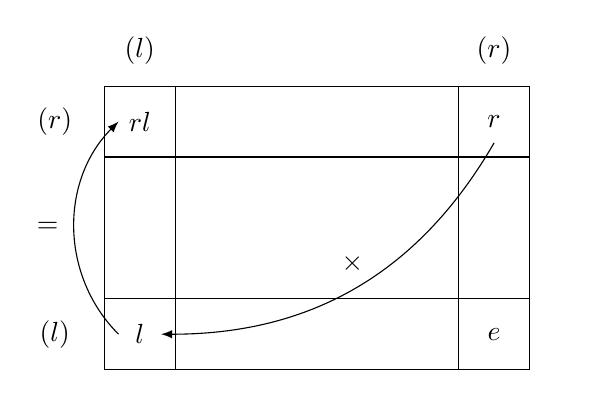
\begin{tikzpicture}[scale = 0.9]
	\tikzstyle{fleche}=[->,>=latex,rounded corners=4pt]
	\node at (0,0){$l$};
	\node at (0,3){$rl$};
	\node at (5,0){$e$};
	\node at (5,3){$r$};
	\draw (-.5,3.5) -- (-.5, -.5);
	\draw (.5,3.5) -- (.5, -.5);
	\draw (5.5,3.5) -- (5.5, -.5);
	\draw (4.5,3.5) -- (4.5, -.5);
	\draw (-.5,3.5) -- (5.5, 3.5);
	\draw (-.5,2.5) -- (5.5, 2.5);
	\draw (-.5,.5) -- (5.5, .5);
	\draw (-.5,-.5) -- (5.5, -.5);
	
	\draw[->, >=latex, bend left = 45] (-.3, 0) to (-.3, 3);
	\node at (-1.3, 1.5){$=$};
	\draw[->, >=latex, bend left] (5,2.7) to (0.3,0);
	\node at (3, 1){$\times$};
	
	\node at (-1.2, 3){$\rc(r)$};
	\node at (-1.2, 0){$\rc(l)$};
	\node at (0, 4){$\lc(l)$};
	\node at (5, 4){$\lc(r)$};
	\node at (6, 0){};
	
	\end{tikzpicture}
	\caption{Location Theorem\\ {\small Since there is an idempotent $e$ in $\lc(r)\cap \rc(l)$, $rl$ stays in the same $\jc$-class, in $\lc(l) \cap \rc(r)$.}}
\end{figure}

\begin{lemme}
	Let $e \in M$ be an idempotent, $R = \rc(e)$ its $\rc$-class and $R'$ another $\rc$-class of $\jc(e)$. Let $(\lambda, \lambda')$ be a left Green pair for $(L, L')$. Then $(\lambda e, e\lambda')$ is a left Green pair for $(R, R')$.
	
	Similarly, if $L = \lc(e)$, $L'$ is a $\lc$-class of $\jc(e)$ and $(\rho, \rho')$ is a right Green pair for $(L, L')$, then $(e\rho, \rho'e)$ is a right Green pair for $(L, L')$
\end{lemme}

\begin{proof}
	Let $g$ be any element of $\hc(e)$ and $g' = \lambda g$. Since $e$ is idempotent, $\hc(e)$ is a group with identity $e$ so we have $e\lambda'\lambda e g = e \lambda'\lambda g = eg = g$ and $\lambda ee\lambda' g' = \lambda eg = \lambda g = g'$ which, from Green's Lemma, make $(\lambda e, e\lambda')$ a left Green pair for $(L, L')$. A similar argument applies for the second part of the proposition.
\end{proof}

\begin{rmk}
	This lemma means that for a regular $\jc$-class $J$ and for any two $\lc$-class (or $\rc$-class) it contains, we may choose a corresponding Green pair among the elements of those two classes.
\end{rmk}

\begin{prop}\label{prop:equations}
	Let $e \in M$ be an idempotent and $H = \hc(e), L = \lc(e), R = \rc(e)$ and $J = \jc(e)$. 
	For each $\rc$-class $R' \subset J$, we choose a left Green pair $(l, l') \in J^2$. We denote by $\mathfrak{L}$ the set of all $l$ for the chosen left Green pairs. We define $\mathfrak{R}$ similarly.
	Then $N_e$ is the set of solutions of :
	\[\forall r \in \mathfrak{R}, \forall g \in H,\quad \sum_{l \in \mathfrak{L}} \ind_H(rl)x_{l(rl)\inv g} = 0\]
\end{prop}

\begin{proof}
	Consider an element $a \in R$. $a$ can be written in a unique way as $gr$, with $g \in G$ and $r \in \mathfrak{R}$ corresponding to $\lc(a)$. Similarly, an element $b$ in $L$ as a unique decomposition as $l\gamma, l \in \mathfrak{L}, \gamma \in H$.
	For an element $x \in \kbf L$ we note:
	\[x = \sum_{l \in \mathfrak{L}, \gamma \in H}x_{l\gamma}l\gamma\]
	its decomposition over the basis $L$.
	
	We want to find the equations that describe $\ker(gr\mul{L})$ (where $gr\mul{L}$ is the linear map on $\kbf L$ obtained by extending the monoid's multiplication by linearity). From the Location Theorem, we get that $\im(gr\mul{L}) \subset \kbf H$.
	For $k \in H$, denote by $f_{k, gr}$ the $k$-th coordinate function of $gr\mul{L}$.
	Because $gr\mul{L}$ acts combinatorially on $\kbf L$, we have :
	\[f_{k, gr}(x) = \sum_{l \in \mathfrak{L}, \gamma \in H} \ind_{\{k\}}(grl\gamma)x_{l \gamma}\]
	
	Note that $x_{l \gamma}$ appears in the sum if and only if $grl\gamma = k$. From the Location Theorem, and because we choose $l \in L, r \in R$, we have $grl\gamma = k \textrm{ if and only if } rl \in H \textrm{ and } \gamma = (rl)\inv g\inv k$
	and thus the equation becomes:
	\[f_{k, gr}(x) = \sum_{l \in \mathfrak{L}} \ind_H(rl)x_{l(rl)\inv g\inv k}.\]
	For $x$ to be in $\ker(gr\mul{L})$, $x$ must cancel simultaneously $f_{k, gr}$ for all $k\in H$. We now have a set of equations for $ker(gr\mul{L})$, and we can deduce that the set of equations
	\[\forall r \in \mathfrak{R}, \forall g,k \in H, \quad f_{k, gr}(x) = \sum_{l \in \mathfrak{L}, \gamma \in H} \ind_H(rl)x_{l (rl)\inv g\inv k} = 0\]
	describes $N_e(\kbf L)$.
	However, the equation system is redundant as the equation $f_{k, gr}(x) = 0$ is the same for all pairs $(g, gk')$ with $k' \in H$. Removing the duplicates equation gives the system announced in the proposition.
\end{proof}

\begin{lined}
	\begin{ex}[$N_e$ in the case of an aperiodic monoid]
		As in Example \ref{ex:aperiodic_bichar}, let us consider the case of a $\jc$-class with trivial $\hc$-classes. In this case, we have $L = \mathfrak{L}, R = \mathfrak{R}$ and $H = \{1_H\}$, so the equations become:
		\[\forall r \in R, \quad \sum_{l\in M}\ind_H(rl)x_l.\]
		Again from the Location Theorem, we have that $\ind_H(rl) = 1$ if and only if there is an idempotent in $\lc(r)\cap\rc(l)$. So if we form a matrix $A$ with rows indexed by $L$ and columns indexed by $R$, and with coefficients 1 at $(\lc(r),\rc(l))$ if $\lc(r)\cap \rc(l)$ contains an idempotent and 0 otherwise, the above equations becomes :
		\[(x_l)_{l\in L}^T A = 0,\]
		that is, in the case of an $\hc$-trivial $\jc$-class, $N_e(\kbf L)$ is the left kernel of the eggbox picture seen as a $\{0, 1\}$-matrix. 
	\end{ex}
\end{lined}

Note that given this set of equations, we can compute the character $\chi_{\kbf M \otimes \kbf G_e^{op}}^{N_e(\kbf\lc(e))}$ from the formula in Proposition \ref{prop:formula_char} using classical linear algebra algorithms to find a basis of $N_e(\kbf\lc(e))$ and then computing the value of the character at any $(m, g) \in C_M \times C_{G_e}$ by iterating over the basis vectors, applying $(m, g)$ as a linear map and computing the relevant coefficient in the image vector.

	
	\section{Performances, computational complexity and benchmarks}\label{sec:perf}
	In this section, we discuss performances in terms of complexity whenever we can, and in terms of benchmarks for timings and memory usage. In the next paragraph, we discuss the challenges in measuring performances and the subsequent choices made. Given these considerations, in the three paragraphs following, we discuss the computationnal performances of our three main objects of interest: the combinatorial bicharacter (\emph{i.e.} fixed-point counting), the character table and finally the Cartan matrix.
	
	\subsection{Discussion and Challenges}\label{sub:challenges}
	\section{Introduction}

The increasing complexity of source code poses a key challenge to the reliability of large-scale software systems. Software bugs in these systems can lead to safety issues~\cite{bug_safety} for users around the world as well as cause non-negligible financial losses~\cite{bug_loss}. As such, developers have to spend a large amount of time and effort on bug fixing. Consequently, \aprfull (\apr), designed to automatically generate patches to fix software bugs, has attracted wide attention from both academia and industry~\cite{long2016prophet, legoues2012genprog, long2015spr, lou2020can, tufano2018empstudy}. 


To achieve \apr, one popular approach is known as Generate-and-Validate (G\&V)~\cite{qi2015gv, ghanbari2019prapr, lou2020can, le2016hdrepair, legoues2012genprog, wen2018capgen, hua2018sketchfix, martinez2016astor, koyuncu2020fixminder, liu2019tbar, liu2019avatar}, which is typically based on the following pipeline: First, fault localization techniques~\cite{wong2016fl, abreu2007ochiai, zhang2013injecting, papadakis2015metallaxis, li2019deepfl, li2017transforming} are applied to determine the suspicious locations in programs where bugs are likely to exist. Then, the buggy locations are used by the \apr tools to generate a list of patches that replace buggy lines with correct lines. Afterward, each patch is validated against the original test suite to identify any \emph{plausible patches} (i.e., passing all tests in the test suite). Finally, to determine the \emph{correct patches}, developers examine the list of plausible patches to see if any of them can correctly fix the bug. 

Traditional \apr tools can mainly be categorized into heuristic-based~\cite{legoues2012genprog, le2016hdrepair, wen2018capgen}, constraint-based~\cite{mechtaev2016angelix, le2017s3, demacro2014nopol, long2015spr} and \template~\cite{ghanbari2019prapr, hua2018sketchfix, martinez2016astor, liu2019tbar, liu2019avatar}. Among these traditional tools, \template \apr tools~\cite{ghanbari2019prapr, liu2019tbar, benton2020effectiveness} have been able to achieve state-of-the-art results. \Template \apr tools typically leverage pre-defined templates (e.g., adding a nullness check) for bug fixing. However, since these fix templates are typically handcrafted, the number and types of bugs they are able to fix can be limited. 



To address the limitations of traditional \apr, researchers have proposed various \learning \apr tools~\cite{li2020dlfix, chen2018sequencer, jiang2021cure, lutellier2020coconut, zhu2021recoder, ye2022rewardrepair} based on the \nmtfull (\nmt) architecture~\cite{sutskever2014mt} where the input is the buggy code snippets and the goal is to translate the buggy code snippets into a fixed version. To accomplish this, \learning \apr tools require supervised training datasets with pairs of both buggy and fixed code snippets in order to learn how to perform this translation step. These training data are usually obtained by mining historical bug fixes using heuristics/keywords~\cite{dallmeier2007benchmark}, which can be imprecise for identifying bug-fixing commits; even the actual bug-fixing commits can include irrelevant code changes, leading to further pollution in the dataset~\cite{xia2022alpharepair}.
% 
Moreover, it can be hard for such \apr tools to generalize and fix bug types unseen during training. 



To better leverage recent advances in \plmfull{s} (\plm{s}), researchers~\cite{xia2022alpharepair, xia2023repairstudy, kolak2022patch, prenner2021codexws} have directly applied \plm{s} to generate patches without bug-fixing datasets. These \llm-based \apr tools work by either directly generating a complete code function~\cite{prenner2021codexws, xia2023repairstudy} or predict/infill the correct code snippet given its surrounding context~\cite{xia2022alpharepair, xia2023repairstudy}. By directly using \llm{s} that are pre-trained on billions of open-source code snippets, \llm-based \apr tools can achieve state-of-the-art performance on many repair datasets~\cite{xia2022alpharepair}. 


% 
%
%

Traditional \apr tools have long used the insight of the \emph{plastic surgery hypothesis}~\cite{barr2014plastic} where it states that the code ingredients to fix a bug already exist within the same project. Traditional \apr tools have manually designed pattern-~\cite{ghanbari2019prapr, saha2017elixir} or heuristic-based~\cite{jiang2018simfix, legoues2012genprog} approaches to finding and using such relevant code ingredients to generate fixes for bugs. However, the plastic surgery hypothesis has been largely ignored in \llm-based \apr. In fact, \llm provides a unique opportunity to fully automate the plastic surgery hypothesis idea via fine-tuning (learning project-specific information via model updates from the buggy project) and prompting (directly providing relevant code ingredients to the model), and make it directly applicable to different languages (since the \llm{s} are typically multi-lingual).%
Moreover, despite the intensive manual efforts involved, traditional \apr tools still cannot fully leverage project-specific information due to large search space for leveraging/composing existing code ingredients. In contrast, the project-specific information can effectively leveraged by \llm{s} due to their power in code understanding/vectorization, e.g., even partial/imprecise information may still guide \llm{s} in correct patch generation!
 To this end, we ask the question: \emph{How useful is the plastic surgery hypothesis in the era of \plm{s}}?








\mypara{Our Work.} To answer the question, we present \ourtech{\xspace} -- a \llm-based approach that automatically utilizes the plastic surgery hypothesis by systematically combining multiple fine-tuning and prompting strategies for \apr. \ourtech fine-tunes \plm{s} using two novel domain-specific training strategies: \textbf{\epfinetune} -- we fine-tune using the original buggy project by aggressively masking out a high percentage of tokens, which allows \plm to learn project-specific code tokens and programming styles; and \textbf{\rofinetune} -- which only masks out a single continuous code sequence per training sample, allowing the model to get used to the final \csapr task of predicting a single continuous code sequence. Furthermore, we directly leverage the ability for \plm{s} to understand natural language instructions and introduce a novel prompting strategy, \textbf{\idprompting}, which uses information retrieval and static analysis to obtain a list of relevant identifiers for the buggy lines. While such relevant identifiers are critical for fixing some difficult bugs, they may not be seen by the \llm during inference due to limited context window size. Through the use of prompting, we directly tell the model to use these extracted identifiers (relevant code ingredients) to generate the correct code. Finally, to perform repair, we combine all four model variants (including the base model, both fine-tuned models and the base model with prompting) for the final repair.





While our insight of leveraging the plastic surgery hypothesis for \llm-based \apr is generalizable across different types of \plm{s}, to implement \ourtech, we choose a recent \plm{\xspace}, \ctfive~\cite{wang2021codet5}, which is pre-trained on millions of open-source code snippets. \ctfive is an encoder-decoder model trained using \mspfull (\msp) objective where a percentage of tokens are masked out and each continuous masked token sequence is referred to as a masked span. Also, although we only extract relevant identifiers from the current buggy project (since this paper focuses on the plastic surgery hypothesis), our work can be easily extended to obtain other code information (such as relevant statements or functions) from other sources, such as  the massive pre-training corpora~\cite{husain2020codesearchnet} or historical bug-fixing datasets~\cite{jiang2019infer}, which can provide more coding knowledge for \llm{s}. Besides, although we mainly focus on using traditional string comparison algorithms for information retrieval in this paper, these techniques can be easily replaced by other frequency-based retrieval~\cite{robertson2009probabilistic} and neural search (or embedding-based search)~\cite{reimers2019sentence}.
  In summary, this paper makes the following contributions:


%


\begin{itemize}[noitemsep, leftmargin=*, topsep=0pt]
    \item \textbf{Dimension.} This paper is the first to revisit the important plastic surgery hypothesis in the era of \llm{s}. It opens up a new dimension for \llm-based \apr to incorporate previously neglected information from the buggy project itself to boost \apr performance. Furthermore, it demonstrates the promising future of retrieval-based prompting for modern \llm-based \apr.
    \item \textbf{Implementation.} We implement \ourtech based on the recent \ctfive model. We augment the model using two novel fine-tuning strategies: \epfinetune and \rofinetune, along with a novel prompting strategy based on information retrieval and static analysis: \idprompting. We combine the patches generated by all four models together and perform patch ranking to speed up \apr.% 
    \item \textbf{Evaluation Study.} We conduct an extensive evaluation against state-of-the-art \apr tools. On the widely studied \dfj 1.2 and 2.0 datasets~\cite{just2014dfj}, \ourtech is able to achieve the new state-of-the-art results of 89 and 44 correct bug fixes (15 and 8 more than best baseline) respectively.  Furthermore, we perform a broad ablation study to justify our design. \ourtech demonstrates for the first time that the plastic surgery hypothesis can substantially boost \llm-based \apr and advance state-of-the-art \apr, while being fully automated and general. Moreover, even partial/imprecise code ingredients may still effectively guide \llm{s} for \apr!
\end{itemize}


	
	\subsection{Fixed point counting}\label{sub:perf_count}
	

Continuing the approach in Section~\ref{sec:counting:preview} for proving equivalence between \AEExactTriCount{} and \AEExactTri{},
we now derive more equivalence results between other counting and detection problems.

\subsection{Min-Plus Product}

In this section, we use $A$ and $B$ to denote the inputs to  a \MinPlus{} or  \MinPlusCount{} instance, and we use $W_{ij}$ to denote the set of $k$ where $A_{ik}+B_{kj} = (A\star B)_{ij}$, i.e., the set of witnesses for $(i, j)$. 

\begin{lemma}
\label{lem:min-plus}
Given two $n \times n$ matrices $A, B$ and a subset $S \subseteq [n]$, we can compute a matrix $D$ in $\OO(|S| \cdot n^{(3+\omega)/2})$ time such that $D_{ij} = |W_{ij}|$ for pairs of $(i, j)$ where $S \cap W_{ij} \ne \emptyset$. 
\end{lemma}
\begin{proof}
For every $s \in S$, we do the following. Let $A^{(s)}$ be a matrix where $A^{(s)}_{ik} = A_{ik} - A_{is}$ and $B^{(s)}_{kj} = B_{sj} - B_{kj}$. Then we  compute the equality product $C^{(s)}$ of $A^{(s)}$ and $B^{(s)}$ in $\OO(n^{(3+\omega)/2})$ time for each $s$ using Matou{\v{s}}ek's algorithm~\cite{MatIPL}. Finally, let $D_{ij}$ be $C^{(s)}_{ij}$ where  $A_{is} + B_{sj}$ is the smallest over all $s \in S$ (breaking ties arbitrarily). The running time for computing $D$ is clearly $\OO(|S| \cdot n^{(3+\omega)/2})$. 

Suppose $S \cap W_{ij} \ne \emptyset$ for some $(i, j)$. Then $D_{ij}$ equals $C^{(s)}_{ij}$ where $A_{is} + B_{sj} = (A \star B)_{ij}$. For any $k$,  $A^{(s)}_{ik} = B^{(s)}_{kj}$ if and only if $A_{ik} + B_{kj} = A_{is} + B_{sj} = (A \star B)_{ij}$ by Fredman's trick. Therefore, $D_{ij} = C^{(s)}_{ij} = |W_{ij}|$.
\end{proof}

\begin{theorem}
\label{thm:minplus-count}
If \MinPlus{} for $n \times n$ matrices has an $O(n^{3-\eps})$ time algorithm for some $\eps > 0$, then \MinPlusCount{} for $n \times n$ matrices  has an $O(n^{3-\eps'})$ time algorithm for some $\eps' > 0$.
\end{theorem}
\begin{proof}
Given a \MinPlusCount{} instance on $n \times n$ matrices $A, B$, we first list up to $n^{0.99}$ elements in $W_{ij}$ for every $i, j$. 
By well-known techniques (e.g.\  \cite{focsyj}), an $O(n^{3-\eps})$ time \MinPlus{} algorithm implies an $O(n^{3-\eps''})$ for $\eps'' > 0$ time algorithm for listing up to $n^{0.99}$ witnesses for each $(i, j)$ in a \MinPlus{} instance. 

If we list less than $n^{0.99}$ elements for some $(i, j)$, then these elements are all the elements in $W_{ij}$. Thus we can output the number of elements we list as the exact witness count for $(i, j)$. For each of the remaining pairs of $(i, j)$, we have found $n^{0.99}$ witnesses. By the standard greedy algorithm for hitting set, in $\OO(n^{2.99})$ time, we can find a set $S$ of size $\OO(n^{0.01})$ that intersects with $W_{ij}$ for each of these remaining $(i, j)$ pairs. Therefore, we can apply Lemma~\ref{lem:min-plus} to compute the number of witnesses for these remaining $(i, j)$ pairs in $\OO(|S| \cdot n^{(3+\omega)/2}) \le O(n^{2.70})$ time. 

The total running time for the \MinPlusCount{} instance is thus $\OO(n^{3-\eps''} + n^{2.99}+n^{2.70})$, which is truly subcubic. 
\end{proof}

We then show the reduction in the other direction. 
The proof is similar to the reduction from a certain version of Min-Plus product to certain versions of  APSP counting in unweighted directed graphs~\cite{CVXicalp21}.
\begin{theorem}
\label{thm:minplus-count-rev}
If \MinPlusCount{} for $n \times n$ matrices has an $O(n^{3-\eps})$ time algorithm for some $\eps > 0$, then \MinPlus{} for $n \times n$ matrices  has an $O(n^{3-\eps'})$ time algorithm for some $\eps' > 0$.
\end{theorem}
\begin{proof}

Let $A, B$ be two $n \times n$ matrices of a \MinPlus{} instance. Let $A'$ be another $n \times n$ matrix where $A'_{ik} = M \cdot A_{ik} + k$ for some large enough integer $M$ (say $M > n$). Similarly, we create an $n \times n$ matrix $B'$ where $B'_{kj} = M \cdot B_{kj}$. This way, for every $i, j$, there exists exactly one $k_{ij}$ such that $A'_{ik_{ij}} + B'_{k_{ij}j} = (A'\star B')_{ij}$. Furthermore, we clearly also have $A_{i,k_{ij}} + B_{k_{ij},j} = (A \star B)_{ij}$. 

Then for each integer $p \in \left[\lceil \log(n) \rceil\right]$, we do the following. Let $A'^{(p)}$ be a copy of $A'$, but we duplicate all columns $k$ where the $p$-th bit in $k$'s binary representation is $1$. We similarly create $B'^{(p)}$ which is a copy of $B'$ but we duplicate all rows $k$ where the $p$-th bit in $k$'s binary representation is $1$. Then we run the $O(n^{3-\eps})$ time  \MinPlusConvCount{} algorithm for $A'^{(p)}$ and $B'^{(p)}$. Suppose for some $i, j$, the number of witnesses is $2$, then we know that the $p$-th bit of  $k_{ij}$ is $1$; otherwise, the $p$-th bit of $k_{ij}$ is $0$. 

After all $\left[\lceil \log(n) \rceil\right]$ rounds, we can compute $k_{ij}$ for every $i, j$. Since $A_{i, k_{ij}} + B_{k_{ij}, j} = (A \star B)_{ij}$, we can then compute the Min-Plus product between $A$ and $B$ in $\OO(n^2)$ time. 
\end{proof}




\subsection{\texorpdfstring{$3$}{3}SUM Convolution and Min-Plus Convolution}
Let $A, B$ and $C$ be the inputs of an \AllThreeSUMConv{} or  \AllThreeSUMConvCount{} instance, and let $W_{k}$ be the set of $i$ where $A_{i}+B_{k-i} =C_{k}$, i.e., the set of witnesses for $k$. 


\begin{lemma}
\label{lem:3sum-conv}
Given a \AllThreeSUMConvCount{} instance for length $n$ arrays $A, B, C$, we can compute $|W_k|$ for every $k$ such that $|W_k| \ge L$ in $\OO(n^{(9+\omega)/4}/L)$ randomized time. 
\end{lemma}
\begin{proof}
First, we find an arbitrary prime $p$ between $2n$ and $4n$, which can be done in $\OO(n)$ time. Also, let $x$ be a uniformly random number sampled from $\mathbb{F}_p \setminus \{0\}$ and let $y$ be a uniformly random number sampled from  $\mathbb{F}_p$. 
Then we create three arrays $A', B'$ and $C'$, indexed by $\mathbb{F}_p$ as follows:
\begin{equation*}
    \begin{split}
        A'_{i} &= \left\{
  \begin{array}{ll}
    A_{x^{-1} (i-y) \bmod{p}} & : x^{-1} (i-y) \bmod{p} \in [n]\\
    M & : \text{otherwise}
  \end{array}
\right.,\\
B'_{i} &= \left\{
  \begin{array}{ll}
    B_{x^{-1} (i+y) \bmod{p}} & :  x^{-1} (i+y) \bmod{p} \in [n]\\
    M & : \text{otherwise}
  \end{array}
\right.,\\
C'_{i} &= \left\{
  \begin{array}{ll}
    C_{x^{-1} i \bmod{p}\phantom{(+y)}}  & :  x^{-1} i \bmod{p} \in [n]\\
    3M & : \text{otherwise}
  \end{array}
\right.,
    \end{split}
\end{equation*}
where $M$ is a large enough number (say $M$ is larger than $10$ times the largest absolute value of the input numbers). 

If we use $W'_k$ to denote the set of $i$ such that $A'_{i} + B'_{(k - i) \bmod{p}} = C'_k$, then it is not difficult to verify that $|W'_{xk \bmod{p}}| = |W_k|$. Thus, from now on, we aim to compute $|W'_k|$ for indices $k$ where $|W'_k| \ge L$. 

We start with the following claim. 
\begin{claim}
\label{cl:3sum-conv-algo}
Let $\mathcal{I} \subseteq \mathbb{F}_p$ be any fixed interval of length $\Theta(\sqrt{n})$ and let $1 \le L' \le \sqrt{n}$ be a fixed value. Then there exists an $\OO(n^{(5+\omega)/4}/L')$ time algorithm that computes $|W_k' \cap \mathcal{I}|$ for every $k$ such that $|W_k' \cap \mathcal{I}| \ge L'$, with high probability. Furthermore, for other values of $k$, we either also compute $|W_k' \cap \mathcal{I}|$ correctly, or declare that we don't know the value of $|W_k' \cap \mathcal{I}|$. 
\end{claim}
\begin{proof}
We first reduce the problem of computing $|W_k' \cap \mathcal{I}|$ to an instance of \AEExactTriCount{}. Similar reductions from convolution problems to matrix-product type problems were known before \cite{bremner2006necklaces, VWfindingcountingj}. Without loss of generality, we assume $\mathcal{I} = \{0, 1, \ldots, \ell - 2, \ell - 1\}$ for some $\ell = \Theta(\sqrt{n})$, by subtracting $\min \mathcal{I}$ from all indices of $A'$ and adding $\min \mathcal{I}$ to all indices of $B'$. 

We then create the following tripartite weighted graph $G$ with three parts $I, J, T$, where $|I| = \ell, |J| = [\lceil p/\ell \rceil]$ and $|T| = 2\ell - 1$. We use $I_i$ to denote the $i$-th node in $I$, $J_j$ to denote the $j$-th node in $J$ and $T_t$ to denote the $t$-th node in $T$. We then add the following edges to the graph: 
\begin{itemize}
    \item For every $i \in [|I|], t \in [|T|]$ such that $i - t + \ell - 1 \in \mathcal{I}$, we add an edge between $I_i$ and $T_t$ with weight $w(I_i, T_t) = A'_{i - t + \ell - 1}$.
    \item For every $t \in [|T|]$ and $j \in [|J|]$, we add an edge between $T_t$ and $J_j$ with weight $w(T_t, J_j) = B'_{((j-1)\ell + t - \ell) \bmod{p}}$. 
    \item For every $i \in [|I|], j \in [|J|]$ such that $(j-1)\ell + i - 1 < p$, we add an edge between $I_i$ and $J_j$ with weight $w(I_i, J_j) = -C'_{(j-1)\ell + i - 1}$. 
\end{itemize}
Consider any $(i, j) \in [\ell] \times [\lceil p/\ell \rceil]$ such that $(j-1)\ell + i - 1 < p$. The nodes $T_t$ such that $i - t + \ell - 1 \in \mathcal{I}$ form triangles with edge $(I_i, J_j)$. The multiset of the weights of these triangles is 
\begin{equation*}
    \begin{split}
        \left\{w(I_i, T_t) + w(J_j, T_t) + w(I_i, J_j) \right\}_{t=i}^{i+\ell-1} &= \left\{A'_{i - t + \ell - 1} + B'_{((j-1)\ell + t - \ell) \bmod{p}} - C'_{(j-1)\ell + i - 1} \right\}_{t=i}^{i+\ell-1}\\
        &= \left\{A'_r + B'_{\left( (j-1)\ell + (i-1) - r\right) \bmod{p}} -C'_{(j-1)\ell + i - 1}\right\}_{r=0}^{\ell - 1}.
    \end{split}
\end{equation*}
Thus, the number of triangles with weight $0$ containing edge $(I_i, J_j)$ in $G$ is exactly  $|W'_k \cap \mathcal{I}|$ for $k = (j-1)\ell + i - 1$.
In particular, if $|W'_k \cap \mathcal{I}| \ge L'$, then the number of witnesses for $(I_i, J_j)$ in the \AEExactTriCount{} instance on graph $G$ and target value $0$ is also at least $L'$. Now let $S$ be a random subset of $V(G)$ of size $C n^{0.5} \log n/L'$ for a sufficiently large constant $C$. Then with high probability, $S$ intersects with the set of witnesses for every edge $(I_i, J_j)$ for which  $k=(j-1)\ell + (i-1)$ has at least $L'$ witnesses in $\mathcal{I}$. Now we can apply Lemma~\ref{lem:exact-tri} on graph $G$, target value $0$ and set $S$ to compute the number of witnesses for these edges $(I_i, J_j)$ in $\OO(|S| \sqrt{n}^{(3+\omega)/2}) = \OO(n^{(5+\omega)/4}/L')$ time. 

If $S$ does not intersect with the witnesses for some edge $(I_i, J_j)$ (which is easy to check in $O(|S|n)$ total time), we declare that we don't know the value of $|W_k' \cap \mathcal{I}|$ for  $k=(j-1)\ell + (i-1)$.
\end{proof}

\begin{claim}
\label{cl:3sum-conv-chebyshev}
Let $\mathcal{I} \subseteq \mathbb{F}_p$ be any fixed interval and $k \in [n]$ be any fixed index. If $|W_k| \ge L$, then 
$$\Pr_{\substack{x \sim \mathbb{F}_p \setminus \{0\} \\ y \sim \mathbb{F}_p}}\left[ \left| W'_{xk \pmod{p}} \cap \mathcal{I} \right| \le \frac{L|\mathcal{I}|}{2p}\right] = O(\frac{n}{L|\mathcal{I}|}).$$
\end{claim}
\begin{proof}
First, note that $W'_{xk \pmod{p}} = \{xw + y \pmod{p}: w \in W_k\}$. Let $X$ be the random variable denoting $\left| W'_{xk \pmod{p}} \cap \mathcal{I}\right|$. First, since for any $w \in W_k$, $xw + y \pmod{p}$ is uniformly at random, $\Pr[xw + y \pmod{p} \in \mathcal{I}] = \frac{|\mathcal{I}|}{p}$, and consequently $\mathbb{E}[X] = \frac{|W_k||\mathcal{I}|}{p}$. 

For any $w, w' \in W_k$ where $w \ne w'$, the probability that both $xw + y \pmod{p}$ and $xw' + y \pmod{p}$ fall in $\mathcal{I}$ can be expressed as
$$\sum_{i_1, i_2 \in \mathcal{I}} \Pr[xw+y \equiv i_1 \pmod{p} \wedge xw'+y \equiv i_2 \pmod{p}]. $$
If $i_1 = i_2$, then $xw+y \equiv i_1 \pmod{p}$ and $xw'+y \equiv i_2 \pmod{p}$ cannot both happen; otherwise, there exists at most one pair $(x, y) \in \mathbb{F}_p \times \mathbb{F}_p$ for which $xw+y \equiv i_1 \pmod{p}$ and $xw'+y \equiv i_2 \pmod{p}$ are both true. Thus, $\Pr[xw + y \pmod{p} \in \mathcal{I} \wedge xw' + y \pmod{p} \in \mathcal{I}] \le \frac{|\mathcal{I}|(|\mathcal{I}|-1)}{p(p-1)} \le \frac{|\mathcal{I}|^2}{p^2}$. Thus, $$\Var[X] = \mathbb{E}[X^2] - \mathbb{E}[X]^2 \le \left(|W_k|(|W_k|-1)\frac{|\mathcal{I}|^2}{p^2} + \mathbb{E}[X] \right)- \mathbb{E}[X]^2 \le \mathbb{E}[X].$$
Also, 
\begin{equation*}
    \Pr\left[X \le \frac{L|\mathcal{I}|}{2p}\right] \le \Pr\left[X \le \frac{|W_k||\mathcal{I}|}{2p}\right] \le \Pr\left[\left|X - \mathbb{E}[X] \right| \le \frac{1}{2} \mathbb{E}[X]\right].
\end{equation*}
By Chebyshev's inequality, this probability can be upper bounded by $\frac{\Var[X]}{(\frac{1}{2} \mathbb{E}[X])^2} = O(\frac{n}{L|\mathcal{I}|})$. 
\end{proof}

We now describe our algorithm for computing $|W_k|$. First, we split $\mathbb{F}_p$ into $\ell = \Theta(\sqrt{n})$ intervals $\mathcal{I}_1, \mathcal{I}_2, \ldots, \mathcal{I}_\ell$, each of size $\Theta(\sqrt{n})$. Then it suffices to compute $|W'_{xk \bmod{p}} \cap \mathcal{I}_i|$ for each $i \in [\ell]$, since $|W_k| = |W'_{xk \bmod{p}}| = \sum_{i=1}^\ell |W'_{xk \bmod{p}} \cap \mathcal{I}_i|$. 

We first run the algorithm in Claim~\ref{cl:3sum-conv-algo} for each $i$ with $L' = \frac{L |\mathcal{I}_i|}{2p}$, which takes $\OO(n^{(5+\omega)/4} / L') = \OO(n^{(7+\omega)/4}/L)$ time. Claim~\ref{cl:3sum-conv-algo}  computes $|W'_{xk \bmod{p}} \cap \mathcal{I}_i|$ as long as $|W'_{xk \bmod{p}} \cap \mathcal{I}_i| \ge L'$. For each fixed $k$, it fails to compute $|W'_{xk \bmod{p}} \cap \mathcal{I}_i|$ with probability $O(\sqrt{n}/L)$ by Claim~\ref{cl:3sum-conv-chebyshev}. For these $k$, we enumerate over $j \in \mathcal{I}_i$, check if $j \in W'_{xk \bmod{p}}$, and then compute  $|W'_{xk \bmod{p}} \cap \mathcal{I}_i|$. In expectation, the cost of these $k$ is $O(\frac{n \cdot \sqrt{n}}{L}  \cdot |\mathcal{I}_i|) = O(n^2 / L)$. 

Summing over all $i \in [\ell]$, the total expected running time of the algorithm is $\OO(n^{(9+\omega)/4}/L)$. 
\end{proof}


\begin{theorem}
\label{thm:all-3sum-conv-count}
If \AllThreeSUMConv{} for length $n$ arrays has an $O(n^{2-\eps})$ time algorithm for some $\eps > 0$, then \AllThreeSUMConvCount{} for length $n$ arrays  has an $O(n^{2-\eps'})$ time randomized algorithm for some $\eps' > 0$
\end{theorem}
\begin{proof}

Similar as before, given an \AllThreeSUMConvCount{} instance on length $n$ arrays $A, B, C$, we can count the number of witnesses for $C_k$ that have at most $n^{0.99}$ witnesses in $O(n^{2-\eps''})$ time by well-known techniques~\cite{focsyj} when \AllThreeSUMConv{} has a truly subquadratic algorithm.




For the rest values of $k$, we run the algorithm in Lemma~\ref{lem:3sum-conv} which runs in $\OO(n^{(9+\omega)/4} / n^{0.99}) = O(n^{1.86})$ time. 

Overall, the algorithm for \AllThreeSUMConvCount{} runs in $O(n^{2-\eps''} + n^{1.86})$ time, which is truly subquadratic. 
\end{proof}

As in Remark~\ref{rem:exact-tri-count}, Theorem~\ref{thm:all-3sum-conv-count} implies that \ThreeSUMConv{} is subquadratically equivalent to \ThreeSUMConvCount{}.

\begin{theorem}
\label{thm:minplus-conv-count}
If \MinPlusConv{} for length $n$ arrays has an $O(n^{2-\eps})$ time algorithm for some $\eps > 0$, then \MinPlusConvCount{} for length $n$ arrays  has an $O(n^{2-\eps'})$ time randomized algorithm for some $\eps' > 0$.
\end{theorem}
\begin{proof}

Given an \MinPlusConvCount{} instance for length $n$ arrays $A, B$, we first run the assumed \MinPlusConv{} algorithm to compute the Min-Plus convolution $C$ of $A$ and $B$ in $O(n^{2-\eps})$ time. 

Similar as before, given the $O(n^{2-\eps})$ time algorithm for \MinPlusConv{}, we can count the number of witnesses for $C_k$ that have at most $n^{0.99}$ witnesses in $O(n^{2-\eps''})$ time by well-known techniques~\cite{focsyj}. 



For the rest values of $k$, we run the algorithm in Lemma~\ref{lem:3sum-conv} with arrays $A, B, C$ and $L = n^{0.99}$ which runs in $\OO(n^{(9+\omega)/4} / n^{0.99}) = O(n^{1.86})$ time. 

Overall, the algorithm for \MinPlusConvCount{} runs in $O(n^{2-\eps}+ n^{2-\eps''} + n^{1.86})$ time, which is truly subquadratic. 
\end{proof}

We then show a reduction from \MinPlusConv{} to \MinPlusConvCount{}. 
\begin{theorem}
\label{thm:minplus-conv-count-rev}
If \MinPlusConvCount{} for length $n$ arrays has an $O(n^{2-\eps})$ time algorithm for some $\eps > 0$, then \MinPlusConv{} for length $n$ arrays  has an $O(n^{2-\eps'})$ time randomized algorithm for some $\eps' > 0$.
\end{theorem}
\begin{proof}
Let $A$ and $B$ be two length $n$ arrays for a \MinPlusConv{} instance. Let $C$ be their Min-Plus convolution. As in proof of Theorem~\ref{thm:minplus-count-rev},
we can assume $|W_k|=1$ for every $k$, i.e., there exists a unique $i_k$ such that $A_{i_k} +B_{k - i_k} = C_k$. 

For each $p \in \left[ \lceil \log(n)\rceil\right]$, we perform the following round. Let $A'$ be a length $2n$ array such that $A'_{2i-1} = A_i$ for every $i \in [n]$, $A'_{2i} = A_i$ for every $i \in [n]$ whose $p$-th bit in its binary representation is $1$, and $A'_{2i} = \infty$ for the rest of $i$. Also, let $B'$ be a length $2n$ array such that $B'_{2i-1} = B'_{2i} = B_i$ for every $i \in [n]$. Now we use the \MinPlusConvCount{} algorithm for arrays $A'$ and $B'$. Suppose $C'$ is the Min-Plus convolution between $A'$ and $B'$. Clearly, for any $k \in [n]$, $C'_{2k-1} = C_k$. Also, suppose $C'_{2k-1}$ has $2$ witnesses, then we know that $A'_{2i_k} = A_{i_k}$ and thus the $p$-th bit in $i_k$-th binary representation is $1$; otherwise the $p$-th bit in $i_k$-th binary representation is $0$. 

Thus, after the $\lceil \log(n)\rceil$ rounds, we can compute $i_k$ for each $k \in [n]$, which can then be used to compute the Min-Plus convolution $C$ between $A$ and $B$ in $O(n)$ time. 
\end{proof}

\subsection{All-Numbers 3SUM}


\begin{theorem}
\label{thm:all-3sum-count}
If \AllThreeSUM{} for  sets of $n$ numbers has an $O(n^{2-\eps})$ time algorithm for some $\eps > 0$, then \AllThreeSUMCount{} for sets of $n$ numbers  has an $O(n^{2-\eps'})$ time randomized algorithm for some $\eps' > 0$.
\end{theorem}
\begin{proof}
If \AllThreeSUM{} for sets of $n$ numbers has an $O(n^{2-\eps})$ time algorithm for $\eps > 0$, then so does \AllThreeSUMConv{} for length $n$ arrays, since \AllThreeSUMConv{} is not harder than \AllThreeSUM{}. Then by Theorem~\ref{thm:all-3sum-conv-count}, \AllThreeSUMConvCount{} for length $n$ arrays has an $O(n^{2-\eps''})$ time algorithm for some $\eps'' > 0$. Therefore, it suffices to reduce \AllThreeSUMCount{} to \AllThreeSUMConvCount{}. Some previous reductions from \ThreeSUM{} to \ThreeSUMConv{} actually work for the counting variants as well~\cite{patrascu2010towards, ChanHe}. Arguably the simplest such reduction is given in~\cite[Section 3]{ChanHe}. Applying their reduction finishes the proof.
\end{proof}










As in Remark~\ref{rem:exact-tri-count}, Theorem~\ref{thm:all-3sum-count} implies that \ThreeSUM{} is subquadratically equivalent to \ThreeSUMCount{}.

Still more equivalence results for other counting and detection problems are given in Appendix~\ref{sec:more_counting}.

\subsection{Discussion}\label{sec:counting:discuss}

Abboud, Feller and Weimann \cite{AbboudFW20} showed that counting the number of Negative Triangles in a graph (even mod 2) can solve \ExactTri, thus presenting a barrier to showing that the Negative Triangle  problem ({\sf Neg-Tri}) is equivalent to its counting variant: Vassilevska W. and Williams \cite{focsyj} showed that {\sf Neg-Tri} is equivalent to \APSP{} under subcubic fine-grained reductions; then if {\sf \#Neg-Tri} can be reduced to {\sf Neg-Tri}, one can also reduce it to \APSP, and since there are fine-grained reductions from \ThreeSUM{}  to \ExactTri{} \cite{VWfindingcountingj}, and from \ExactTri{} to {\sf \#Neg-Tri} \cite{AbboudFW20}, one would get a very surprising reduction from \ThreeSUM{} to \APSP. There is some evidence that such a reduction would be difficult to obtain: for instance, while \APSP{} has a superlogarithmic improvement over its simple cubic algorithm \cite{Williams18}, the best improvement over the simple quadratic algorithm of \ThreeSUM{} only shaves two logarithmic factors (e.g. \cite{baran2005subquadratic})!

Our equivalences between \MinPlus{} (and thus Minimum Weight Triangle) and \ExactTri{} respectively with their counting variants exhibit a strange phenomenon: {\sf Neg-Tri} seems different from these problems! Or, perhaps, if we believe that {\sf Neg-Tri} is like these problems and is equivalent to {\sf \#Neg-Tri}, then we should be more optimistic about the existence of a fine-grained reduction from \ThreeSUM{} to \APSP.


Another line of work in which counting variants of fine-grained problems have been considered is in worst-case to average-case reductions and {\em fine-grained cryptography} \cite{BallRSV17,BallRSV18,Boix-AdseraBB19,GO2020,DalirrooyfardLW20,LaVigneLW19,merkle}: building cryptographic primitives from worst-case fine-grained assumptions that might still hold even if $\text{P}=\text{NP}$. The known techniques 
 for worst-case to average-case reductions for fine-grained problems only work for counting problems, whereas the design of fine-grained public key protocols \cite{LaVigneLW19,merkle} seem to require that the decision variants are hard on average.





Suppose that one can use the known toolbox for worst-case to average-case reductions for counting problems to show that \ExactTriCount{} or \ThreeSUMCount{} is hard on average.
Then via our reductions back to \ExactTri{} and \ThreeSUM{}, one would get some distributions for which these decision problems are actually hard. This could pave the way to new public-key protocols.

	
	\subsection{Character table}\label{sub:perf_table}
	\setlength{\tabcolsep}{2.5pt}
\begin{table*}[t]
\small
\centering
\caption{Experimental results of proposed method.}
\begin{tabular}{lcccccccccccccccclccccc}
\hline
                              &  &               &              &  & \multicolumn{7}{c}{Total   Power Consumption {[}mW{]}}                &  & \multicolumn{2}{c}{}          &  &                                                                           &  & \multicolumn{1}{l}{}                                                            \\ \cline{6-12}
                              &  & \multicolumn{2}{c}{Accuracy} &  &
			      \multicolumn{3}{c}{Standard HW} &  &
			      \multicolumn{3}{c}{Optimized HW} &  &
			      \multicolumn{2}{c}{\#Selected} &  &
			      \multirow{2}{*}{\begin{tabular}[c]{@{}c@{}}Max
				Delay\\ Red.\end{tabular}} &  &
				\multirow{2}{*}{\begin{tabular}[c]{@{}c@{}}Voltage
				  Scaling\\ Factor\end{tabular}} &
				  \multirow{2}{*}{\begin{tabular}[c]{@{}c@{}}
				    \\ V\_SHW\end{tabular}} &
				    \multirow{2}{*}{\begin{tabular}[c]{@{}c@{}}\\
				    V\_OHW\end{tabular}}\\ \cline{3-4} \cline{6-8} \cline{10-12} \cline{14-15}
Network-Dataset               &  & Orig.         & Prop.        &  & Orig.   & Prop.     & Red.      &  & Orig.   & Prop.     & Red.      &  & Wei.            & Act.          &  &                                                                           &  &                                                                                 \\ \hline
LeNet-5-CIFAR-10              &  & 80.6\%        & 78.5\%       &  & 375.5   & 149.6   & 60.2\%  &  & 360.7    & 78.3    & 78.3\%  &  & 35            & 210           &  & 40 ps                                                                    &  & 0.71/0.8  & 10.1\%  & 5.4\%                                                                       \\
ResNet-20-CIFAR-10            &  & 91.9\%        & 89.6\%       &  & 718.9   & 361.0   & 49.8\%  &  & 663.9    & 288.3   & 56.6\%  &  & 35            & 210           &  & 40 ps                                                                    &  & 0.71/0.8    & 13.2\%  & 11.5\%                                                                     \\
ResNet-50-CIFAR-100           &  & 79.9\%        & 78.5\%       &  & 708.7   & 293.8   & 58.5\%  &  & 701.8    & 157.1   & 77.6\%  &  & 41            & 223           &  & 30 ps                                                                    &  & 0.73/0.8  & 8.1\%  & 4.2\%                                                                      \\
EfficientNet-B0-Lite-ImageNet &  & 73.8\%        & 69.7\%       &  & 21.2    & 19.3    & 9.0\%   &  & 2.4      & 1.9     & 20.8\%  &  & 50            & 236           &  & 20 ps                                                                    &  & 0.75/0.8  & 6.4\%  & 6.5\%                                                                      \\ \hline
\end{tabular}
\label{tab:results}
\end{table*}





	
	\subsection{Cartan matrix}\label{sub:perf_cartan}
	We are, at last, in measure to state the formula from Thiéry for the Cartan Matrix. Without getting into the specific details, the Cartan matrix can be seen as measure of how "not semi-simple" the algebra of the monoid is. 
We use a non standard definition of the Cartan matrix, first given in \cite[Definition 2.6]{Thiery.CartanMatrixMonoid}. A formal proof that this is equivalent to the usual definition can be found in \cite[Corolary 7.28]{steinberg2016representation}.

\begin{dftn}
	Let $\{S_1, \dots, S_n\}$ be a set of representatives of the isomorphism classes of simple $\kbf M$-modules. The simple $\kbf M \otimes \kbf M^{op}$ modules are the $S_i \otimes S_j^*$ for all $i, j \in \intint{1, n}$. Denote by $[\kbf M : S_i \otimes S_j^*]$ the multiplicity of $S_i \otimes S_j^*$ as a composition factor of $\kbf M$.
	
	The Cartan matrix of $\kbf M$ is defined by:
	\[C(\kbf M) = ([\kbf M : S_i \otimes S_j^*])_{i, j}\] 
\end{dftn}

In other words, the Cartan matrix is a recording of the multiplicities of the composition factors of $\kbf M$ as a $\kbf M \otimes \kbf M^{op}$ module. But so is its character! The difference being that the character of $\kbf M$ as it is computed is expressed in the basis of the character equivalency classes of $M \times M^{op}$ while the Cartan matrix is expressed directly in the basis of the simple modules. Since the basis change between the two is precisely given by the character table and hence, we have the Thiéry's Formula for the Cartan matrix.

\begin{prop}\label{prop:formule_cartan}
	The Cartan matrix is given by the formula:
	\[C(\kbf M) = {}^tX_M\inv B X_M\inv\]
	where $B = (|\{s \in M \sepp msm'\}|)_{m,m' \in C_M}$
\end{prop}
	
	\section*{Conclusion and perspectives}

	The methods presented in this paper provide a new tool for the computational exploration of finite monoids representation theory. We give a method to compute the character table of a finite monoid in the general case as well as a method for the computation of the Cartan matrix. In the latter case, although general algorithms for any finite dimensional algebra already exist, by specializing to monoid algebras, we achieve vastly shorter computation times, thus making the question tractable for bigger monoids. Although we have presented the methods in details only for transformation monoids, the underlying formulas are true in general for finite monoids, and it remains computationally applicable whenever wherever the hypotheses of Section \ref{sec:Algos} are verified. We also invite the reader the consult and test our impementation, available on our github repository\footnote{github.com/ZoltanCoccyx/monoid-character-table}. As this paper is inspired by the combinatorial research on monoid representation theory which have seen renewed activity in recent years we hope that providing this effective tool will allows for the observation of new phenomena.
	
	This work has two natural continuations: improving and expanding.
	For the improvement part, we have noted that by far the most inefficient part of our algorithm is the computation of the radical of the $\lc$-classes, which happens to be the only point where linear algebra is necessary and combinatorics are seemingly not enough. 
	We can ask whether this step could be replaced by a combinatorial computation. 
	Some experiments show that, even in relatively small and very regular cases ($T_5$ for instance) the basis we find for the radical by solving the equation system described in Proposition \ref{prop:equations} does not have easily understandable structure, once the common denominator of the coefficients is eliminated. It therefore seem unlikely to us that a general method for computing the radical of an entirely combinatorial nature exists, although we remain optimistic that in very regular cases (again, $T_n$), the issue lies with us not finding the method rather than it not existing.
	More modestly, in a general context, we could try to exploit further the structure of the equations that define the radical to reduce the size of the system, which is a major bottleneck.

	Another improvement, although perhaps less impactful, could be made by exploiting redundancy: it can happen that two $\lc$-classes $L_1, L_2$ of a submonoid $M$ of $T_n$ are contained in the same $\lc$-class $L$ of $T_n$. Thus, in step $2-b$ of Algorithm \ref{algo:j_class} (for instance), instead of visiting each $\lc$ of $M$, we could visit each $\lc$ of $T_n$ that contain an $\lc$-class of $M$ and count them with some multiplicity. Although this probably would not lead to great improvements in efficiency, this has the advantage of making, in some sense, $T_n$ the worst case scenario, allowing for a finer complexity analysis.
	
	As for extending this work, the natural path seem to adapt these methods for fields of finite characteristic. At this point it appears to us that this question is tractable as the theory remains essentially the same, although it is somewhat difficult to implement in practice. The main hurdle arise, again, when computing the radical of an $\lc$-class: an equivalent of Proposition \ref{prop:rad_is_ne} would have to take into account the role of the radical of the maximal subgroup algebra, which can be non-trivial in positive characteristic. This would translate in needing to effectively compute this radical. Although algorithms are available (for instance in GAP), this is a theoretically difficult and computationally expensive problem, considerably reducing the maximum size of a tractable problem. While modular representation theory is known to be a difficult subject in groups it seems that, again, the situation is not much more complicated for monoids than it is for groups as it is standard practice to reduce monoid theoretic questions to group theoretic ones. Treating modular group representation theory as a black box coming with already existing algorithms (much as we did here for null characteristic group representation theory as a matter of fact), we hope to be able to provide a modular version of our algorithms along with an implementation in the near future.
	
	\section*{Acknowledgements}
	The research work devoted to this project was funded by a PhD grant from the French \emph{Ministère de la recherche et de l'enseignement supérieur}, in the form of a \emph{Contrat Doctoral Spécifique Normalien} attributed for a PhD in the STIC (\emph{Sciences et Technologies de l'Information et de la Communication}) doctoral school of Paris-Saclay University, in the LISN (\emph{Laboratoire Interdisciplinaire des Sciences du Numérique}) under the supervision of Pr. Nicolas Thiéry.
	
	\clearpage
	
	%\bibliographystyle{abbrv}
	
	%\bibliography{biblio}
	\printbibliography
	
\end{document}
